\documentclass[twoside,11pt,a4paper,openany]{book}
\usepackage[amsbb,subscriptcorrection,zswash,mtpcal,mtphrb]{mtpro2}
\usepackage[no-math,cm-default]{fontspec}
\usepackage{xunicode}
\usepackage{xgreek}
\defaultfontfeatures{Mapping=tex-text,Scale=MatchLowercase}
\def\xrwma{black}
\def\xrwmath{black}
\setmainfont[Mapping=tex-text,Numbers=Lining,Scale=1.0]{Nimbus Roman}
\usepackage{fontawesome5}
%\newfontfamily{\FA}{fontawesome.otf}
\usepackage{amsmath}
\usepackage[left=2.00cm, right=2.00cm, top=3.00cm, bottom=2.00cm]{geometry}
\usepackage{makeidx}
\usepackage{longtable}
\usepackage{etoolbox}
\makeatletter
\newif\ifLT@nocaption
\preto\longtable{\LT@nocaptiontrue}
\appto\endlongtable{%
\ifLT@nocaption
\addtocounter{table}{\m@ne}%
\fi}
\preto\LT@caption{%
\noalign{\global\LT@nocaptionfalse}}
\makeatother
\makeindex
\usepackage{tikz,pgfplots}
\usepackage{tkz-euclide,tkz-fct}
\usepackage{wrapfig}
\usepackage{calc}
\usepackage[colorlinks=false, pdfborder={0 0 0}]{hyperref}
\usepackage{cleveref}
\usepackage[framemethod=TikZ]{mdframed}
\newcommand{\ypogrammisi}[1]{\underline{\smash{#1}}}
\usetikzlibrary{backgrounds}
\renewcommand{\thepart}{\arabic{part}}
\definecolor{steelblue}{cmyk}{.7,.278,0,.294}
\definecolor{doc}{cmyk}{1,0.455,0,0.569}
\definecolor{olivedrab}{cmyk}{0.25,0,0.75,0.44}
\usepackage{capt-of}
\usepackage{titletoc}
\usepackage[explicit]{titlesec}
\usepackage{graphicx}
\usepackage{multicol}
\usepackage{multirow}
\usepackage{enumitem}
\usepackage{tabularx}
\usepackage{mathimatika,tkz-tab,gensymb}
\tikzset{>=latex}
\makeatletter
\pretocmd{\@part}{\gdef\parttitle{#1}}{}{}
\pretocmd{\@spart}{\gdef\parttitle{#1}}{}{}
\makeatother
\usepackage[titletoc]{appendix}
\usepackage{fancyhdr}
\pagestyle{fancy}
\fancyheadoffset{0cm}
\renewcommand{\headrulewidth}{\iftopfloat{0pt}{.5pt}}
\renewcommand{\chaptermark}[1]{\markboth{#1}{}}
\renewcommand{\sectionmark}[1]{\markright{\it\thesection\ #1}}
\fancyhf{}
\fancyhead[LE]{\thepage\ $\cdot$\ \scshape\nouppercase{\leftmark}}
\fancyhead[RO]{\nouppercase{\rightmark} $\cdot$\ \thepage}
\fancypagestyle{plain}{%
\fancyhead{} %
\renewcommand{\headrulewidth}{0pt}}

\newcounter{thewrhma}[chapter]
\renewcommand{\thethewrhma}{\thechapter.\arabic{thewrhma}} 
\newcommand{\Thewrhma}[1]{\refstepcounter{thewrhma}{\textbf{\textcolor{\xrwmath}{{\large Θεώρημα\hspace{2mm}\thethewrhma\;}:\;}\hspace{1mm}}} \MakeUppercase{\textbf{#1}}\\}{}

\newcounter{porisma}[chapter]
\renewcommand{\theporisma}{\thechapter.\arabic{porisma}}\newcommand{\Porisma}[1]{\refstepcounter{porisma}\textcolor{black}{\textbf{ΠΟΡΙΣΜΑ\hspace{2mm}\theporisma\hspace{1mm} \MakeUppercase{#1}}}\\}{}

\newcounter{protasi}[chapter]
\renewcommand{\theprotasi}{\thechapter.\arabic{protasi}}\newcommand{\Protasi}[1]{\refstepcounter{protasi}\textcolor{black}{\textbf{ΠΡΟΤΑΣΗ\hspace{2mm}\theprotasi\hspace{1mm} \MakeUppercase{#1}}}\\}{}

\newcounter{methodologia}[chapter]
\renewcommand{\themethodologia}{\thechapter.\arabic{methodologia}}\newcommand{\Methodologia}[1]{\refstepcounter{methodologia}\textcolor{black}{\textbf{MΕΘΟΔΟΣ\hspace{2mm}\themethodologia\hspace{1mm} \MakeUppercase{#1}}}\\}{}

\newcounter{orismos}[chapter]
\renewcommand{\theorismos}{\arabic{orismos}}   
\newcommand{\Orismos}[1]{\refstepcounter{orismos}{\textbf{\textbf{\textcolor{\xrwma}{{\large Ορισμός\hspace{2mm}\thechapter.\theorismos\;}:\;}}}}\hspace{1mm} \MakeUppercase{\textbf{#1}\\}}{}
\usepackage{venndiagram}
%-------- ΣΤΥΛ ΚΕΦΑΛΑΙΟΥ ---------
\newcommand*\chapterlabel{}
\newcommand{\fancychapter}{%
\titleformat{\chapter}
{
\normalfont\Huge}
{\gdef\chapterlabel{\thechapter\ }}{0pt}
{\begin{tikzpicture}[remember picture,overlay]
\node[yshift=-7cm] at (current page.north west)
{\begin{tikzpicture}[remember picture, overlay]
%\node[inner sep=0pt] at ($(current page.north) +			(0cm,-1.38in)$) {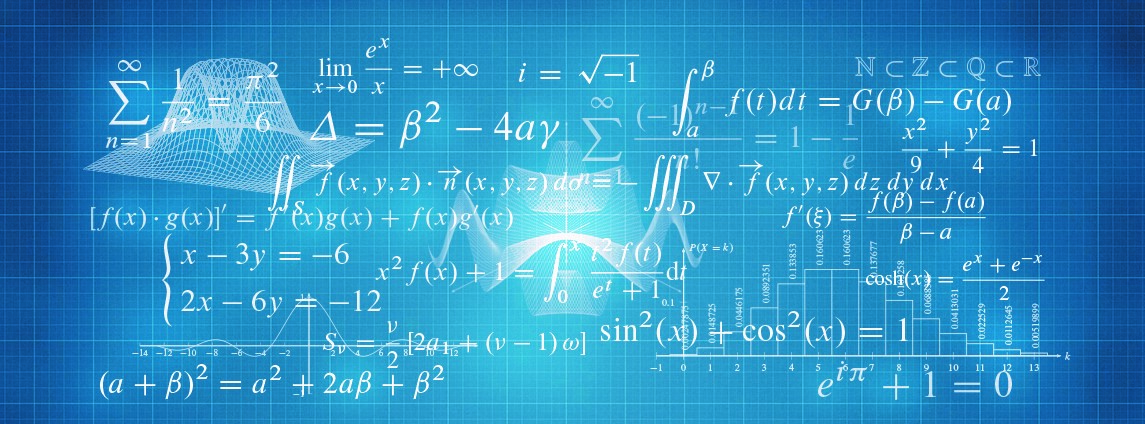
\includegraphics[width=17cm]{Kefalaio}};
\node[anchor=west,xshift=.08\paperwidth,yshift=.1\paperheight,rectangle]
{{\color{white}\fontsize{30}{20}\textbf{\textcolor{black}{\contour{white}{ΚΕΦΑΛΑΙΟ}}}}};
\node[anchor=west,xshift=.07\paperwidth,yshift=.05\paperheight,rectangle] {\fontsize{27}{20} {\color{black}{{\textcolor{black}{\contour{white}{\sc##1}}}}}};
%\fill[fill=black] (12.2,2) rectangle (14.8,4.7);
\node[anchor=west,xshift=.77\paperwidth,yshift=.077\paperheight,rectangle]
{\fontsize{80}{20}\textbf{\textit{\contour{black}{\thechapter}}}};
\end{tikzpicture}
};
\end{tikzpicture}
}
\titlespacing*{\chapter}{0pt}{20pt}{30pt}
}
%------------------------------------------------

\usepackage[outline]{contour}
\newcommand{\regularchapter}{%
\titleformat{\chapter}[display]
{\normalfont\huge\bfseries}{\chaptertitlename\ \thechapter}{20pt}{\Huge##1}
\titlespacing*{\chapter}
{0pt}{-20pt}{40pt}
}

\apptocmd{\mainmatter}{\fancychapter}{}{}
\apptocmd{\backmatter}{\regularchapter}{}{}
\apptocmd{\frontmatter}{\regularchapter}{}{}

\titlespacing*{\section}
{0pt}{30pt}{0pt}
\usepackage{booktabs}
\usepackage{hhline}
\DeclareRobustCommand{\perthousand}{%
\ifmmode
\text{\textperthousand}%
\else
\textperthousand
\fi}

\newcounter{typos}[chapter]
\renewcommand{\thetypos}{T\arabic{typos}}   
\newcommand{\Typos}{\refstepcounter{typos}\textcolor{gray}{\textbf{\thetypos}}}{}


\contentsmargin{0cm}
\titlecontents{part}[-1pc]
{\addvspace{10pt}%
\bf\Large ΜΕΡΟΣ\quad }%
{}
{}
{\;\dotfill\;\normalsize\ Σελίδα}%
%------------------------------------------
\titlecontents{chapter}[0pc]
{\addvspace{30pt}%
\begin{tikzpicture}[remember picture, overlay]%
\draw[fill=black,draw=black] (-.3,.5) rectangle (3.7,1.1); %
\pgftext[left,x=0cm,y=0.75cm]{\color{white}\sc\Large\bfseries Κεφάλαιο\ \thecontentslabel};%
\end{tikzpicture}\large\sc}%
{}
{}
{\hspace*{-2.3em}\hfill\normalsize Σελίδα \thecontentspage}%
\titlecontents{section}[2.4pc]
{\addvspace{1pt}}
{\contentslabel[\thecontentslabel]{2pc}}
{}
{\;\dotfill\;\small \thecontentspage}
[]
\titlecontents*{subsection}[4pc]
{\addvspace{-1pt}\small}
{}
{}
{\ --- \small\thecontentspage}
[ \textbullet\ ][]

\makeatletter
\renewcommand{\tableofcontents}{%
\chapter*{%
\vspace*{-20\p@}%
\begin{tikzpicture}[remember picture, overlay]%
\pgftext[right,x=12cm,y=0.2cm]{\Huge\sc\bfseries \contentsname};%
\draw[fill=black,draw=black] (9.5,-.75) rectangle (12.5,1);%
\clip (9.5,-.75) rectangle (15,1);
\pgftext[right,x=12cm,y=0.2cm]{\color{white}\Huge\bfseries \contentsname};%
\end{tikzpicture}}%
\@starttoc{toc}}
\makeatother
\pgfmathdeclarefunction{gauss}{2}{%
\pgfmathparse{1/(#2*sqrt(2*pi))*exp(-((x-#1)^2)/(2*#2^2))}%
}
\usepackage[contents={},scale=1,opacity=1,color=black,angle=0]{background}

\newcommand\blfootnote[1]{%
\begingroup
\renewcommand\thefootnote{}\footnote{#1}%
\addtocounter{footnote}{-1}%
\endgroup
}
\usepackage{epstopdf}
\epstopdfsetup{update}
\usepackage{textcomp}
\titleformat{\section}
{\normalfont\Large\bf}%
{}{0em}%
{{\color{black}\titlerule[1pt]}\vskip-.2\baselineskip{\parbox[t]{\dimexpr\textwidth-2\fboxsep\relax}{\raggedright\strut\thesection~#1\strut}}}[\vskip 0\baselineskip{\color{black}\titlerule[1pt]}]
\titlespacing*{\section}{0pt}{0pt}{0pt}

\newcommand{\methodologia}{\begin{center}
{\large \textbf{ΜΕΘΟΔΟΛΟΓΙΑ}}\\\vspace{-2mm}
\begin{tikzpicture}
\shade[left color=white, right color=black] (-3cm,0) rectangle (0,.2mm);
\shade[left color=black, right color=white] (0,0) rectangle (3cm,.2mm);   
\end{tikzpicture}
\end{center}}

\newcommand{\orismoi}{\begin{center}
\large \textcolor{\xrwma}{\textbf{ΟΡΙΣΜΟΙ}}\\\vspace{-2mm}
\begin{tikzpicture}
\shade[left color=white, right color=\xrwma] (-3cm,0) rectangle (0,.2mm);
\shade[left color=\xrwma, right color=white] (0,0) rectangle (3cm,.2mm);   
\end{tikzpicture}
\end{center}}
\newcommand{\thewrhmata}{\begin{center}
{\large \textcolor{\xrwmath}{\textbf{ΘΕΩΡΗΜΑΤΑ - ΠΟΡΙΣΜΑΤΑ - ΠΡΟΤΑΣΕΙΣ\\ΚΡΙΤΗΡΙΑ - ΙΔΙΟΤΗΤΕΣ}}}\\\vspace{-2mm}
\begin{tikzpicture}
\shade[left color=white, right color=\xrwmath,] (-5cm,0) rectangle (0,.2mm);
\shade[left color=\xrwmath, right color=white,] (0,0) rectangle (5cm,.2mm);   
\end{tikzpicture}
\end{center}}
\usepackage[labelfont={footnotesize,it,bf},font={footnotesize}]{caption}

\usepackage{wrapfig,wrap-rl}
%-------- ΜΑΘΗΜΑΤΙΚΑ ΕΡΓΑΛΕΙΑ ---------
\usepackage{mathtools}
%----------------------
%-------- ΠΙΝΑΚΕΣ ---------
\usepackage{booktabs}
%----------------------
%----- ΥΠΟΛΟΓΙΣΤΗΣ ----------
%\usepackage{calculator}
%----------------------------
\newcommand{\tss}[1]{\textsuperscript{#1}}
\newcommand{\tssL}[1]{\MakeLowercase{\textsuperscript{#1}}}
%----- ΟΡΙΖΟΝΤΙΑ ΛΙΣΤΑ ------
\usepackage{xparse}
\newcounter{answers}
\renewcommand\theanswers{\arabic{answers}}
\ExplSyntaxOn
\NewDocumentCommand{\results}{m}
{
\seq_set_split:Nnn \l_results_a_seq {,}{#1}
\par\nobreak\noindent\setcounter{answers}{0}
\seq_map_inline:Nn \l_results_a_seq
{
\makebox[.18\linewidth][l]{\stepcounter{answers}\theanswers.~##1}\hfill
}
\par
}
\seq_new:N \l_results_a_seq
\ExplSyntaxOff
%----------------------------

\usepackage{microtype}
\usepackage{float}
\usepackage{caption}
%----------- ΓΡΑΦΙΚΕΣ ΠΑΡΑΣΤΑΣΕΙΣ ---------
\pgfkeys{/pgfplots/aks_on/.style={axis lines=center,
xlabel style={at={(current axis.right of origin)},xshift=1.5ex, anchor=center},
ylabel style={at={(current axis.above origin)},yshift=1.5ex, anchor=center}}}
\pgfkeys{/pgfplots/grafikh parastash/.style={\xrwma,line width=.4mm,samples=200}}
\pgfkeys{/pgfplots/belh ar/.style={tick label style={font=\scriptsize},axis line style={-latex}}}
%-----------------------------------------


\tikzstyle{pl}=[line width=0.3mm]
\tikzstyle{plm}=[line width=0.4mm]
\tkzSetUpPoint[size=2.7,fill=white]
\newlist{rlist}{enumerate}{3}
\setlist[rlist]{itemsep=0mm,label=\roman*.}
\setlist[itemize]{itemsep=0mm}
\definecolor{bblue}{HTML}{4F81BD}
\definecolor{rred}{HTML}{C0504D}
\definecolor{ggreen}{HTML}{9BBB59}
\definecolor{ppurple}{HTML}{9F4C7C}

\makeatletter
\usetikzlibrary{patterns}
\tikzstyle{chart}=[
legend label/.style={font={\scriptsize},anchor=west,align=left},
legend box/.style={rectangle, draw, minimum size=5pt},
axis/.style={black,semithick,->},
axis label/.style={anchor=east,font={\tiny}},
]

\tikzstyle{bar chart}=[
chart,
bar width/.code={
\pgfmathparse{##1/2}
\global\let\bar@w\pgfmathresult
},
bar/.style={very thick, draw=white},
bar label/.style={font={\bf\small},anchor=north},
bar value/.style={font={\footnotesize}},
bar width=.75,
]

\tikzstyle{pie chart}=[
chart,
slice/.style={line cap=round, line join=round,thick,draw=white},
pie title/.style={font={\bf}},
slice type/.style 2 args={
##1/.style={fill=##2},
values of ##1/.style={}
}
]

\pgfdeclarelayer{background}
\pgfdeclarelayer{foreground}
\pgfsetlayers{background,main,foreground}


\newcommand{\pie}[3][]{
\begin{scope}[#1]
\pgfmathsetmacro{\curA}{90}
\pgfmathsetmacro{\r}{1}
\def\c{(0,0)}
\node[pie title] at (90:1.3) {#2};
\foreach \v/\s/\l in{#3}{
\pgfmathsetmacro{\deltaA}{\v/100*360}
\pgfmathsetmacro{\nextA}{\curA + \deltaA}
\pgfmathsetmacro{\midA}{(\curA+\nextA)/2}

\path[slice,\s] \c
-- +(\curA:\r)
arc (\curA:\nextA:\r)
-- cycle;
\pgfmathsetmacro{\d}{max((\deltaA * -(.5/50) + 1) , .5)}

\begin{pgfonlayer}{foreground}
\path \c -- node[pos=\d,pie values,values of \s]{$\l$} +(\midA:\r);
\end{pgfonlayer}

\global\let\curA\nextA
}
\end{scope}
}

\newcommand{\legend}[2][]{
\begin{scope}[#1]
\path
\foreach \n/\s in {#2}
{
++(0,-10pt) node[\s,legend box] {} +(5pt,0) node[legend label] {\n}
}
;
\end{scope}
}
\definecolor{a}{cmyk}{0,1,1,0.05}
\definecolor{b}{cmyk}{0,.8,.8,.15}
\definecolor{c}{cmyk}{0,.8,.8,.0}
\definecolor{d}{cmyk}{0,.7,.7,0}
\definecolor{e}{cmyk}{0,.5,.5,0}


\pgfplotsset{every axis/.append style={
x tick label style={/pgf/number format/.cd, 1000 sep={.}}}}
\newcommand{\shmeio}[2]{
\foreach \a in {1,...,#2}{
\node[dot] at (#1+.5,\a/2-.2){};}}


\newfontfamily\scfont{GFS Artemisia}
\font\mymath = "MyMathSymbols"
\newcommand{\titlos}[3]{
\begin{center}
{\begin{figure}[h]
\centering

\includegraphics[width=0.4\linewidth]{C:/texlive/texmf-local/tex/latex/local/frontisthrio/Logotypo-Filomatheia_1.eps}\ \ \ \ \  
\end{figure}}\vspace{-3mm}
\rule{14.7cm}{.1mm}\\
\vspace{2mm}
ΣΗΜΕΙΩΣΕΙΣ ΜΑΘΗΜΑΤΟΣ - ΘΕΩΡΙΑ, ΜΕΘΟΔΟΛΟΓΙΑ ΚΑΙ ΛΥΜΕΝΕΣ ΑΣΚΗΣΕΙΣ\\
\vspace{1mm}
{\bf\today}
\end{center}
\vspace{.5cm}
\begin{center}
{\Large\bf\MakeUppercase{#1}}
\end{center}
\begin{center}
\textbf{{\Huge \textcolor{black}{#2}}}
\end{center}
\vspace{-1mm}
\begin{center}
{\Large\bf{\MakeUppercase{#3}}}
\end{center}
\vspace{1cm}}

\DeclareMathSizes{10.95}{10.95}{7}{5}
\DeclareMathSizes{6}{6}{3.8}{2.7}
\DeclareMathSizes{8}{8}{5.1}{3.6}
\DeclareMathSizes{9}{9}{5.8}{4.1}
\DeclareMathSizes{10}{10}{6.4}{4.5}
\DeclareMathSizes{12}{12}{7.7}{5.5}
\DeclareMathSizes{14.4}{14.4}{9.2}{6.5}
\DeclareMathSizes{17.28}{17.28}{11}{7.9}
\DeclareMathSizes{20.74}{20.74}{13.3}{9.4}
\DeclareMathSizes{24.88}{24.88}{16}{11.3}

\makeatletter
\AtBeginDocument{
\check@mathfonts
\fontdimen16\textfont2=2.5pt
\fontdimen17\textfont2=2.5pt
\fontdimen14\textfont2=4.5pt
\fontdimen13\textfont2=4.5pt 
}
\makeatother



\begin{document}
\pagenumbering{gobble}% Remove page numbers (and reset to 1)
\clearpage
\backmatter
\pagestyle{empty}
%\titlos{ΑΛΓΕΒΡΑ}{Β Λυκείου}{Ορισμοί και θεωρήματα}
\vspace{1cm}
\begin{center}
\begin{tikzpicture}
\draw[shift={(2.8mm,3.5mm)},style=help lines, xstep=0.5497cm,ystep=0.297cm,black!10] (0,0) grid (8.796,2.38);
\begin{axis}[x=.7cm,y=.7cm,xtick={
-6.28318, -4.7123889, -3.14159, -1.5708,
1.5708, 3.14159, 4.7123889, 6.28318,7.854,9.424,10.995,12.564},
xticklabels={
$-2\pi$, $-\frac{3\pi}{2}$, $-\pi$, $\frac{\pi}{2}$,
$\frac{\pi}{2}$, $\pi$, $\frac{3\pi}{2}$, $2\pi$,$\frac{5\pi}{2}$,$3\pi$,$\frac{7\pi}{2}$,$4\pi$
},ytick={-1.7,-.85,0.85,1.7},yticklabels={$-1$,$-0.5$,$0.5$,$1$},aks_on,xmin=-.4,xmax=13.2,
ymin=-2.2,ymax=2.2,xlabel={\footnotesize $ x $},
ylabel={\footnotesize $ y $},belh ar,clip=false]
\addplot[grafikh parastash,domain=0:2*pi]{1.7*sin(deg(x))};
\addplot[grafikh parastash,domain=2*pi:4*pi,dashed]{1.7*sin(deg(x))};
\end{axis}
\node at (0.0951,1.344) {\footnotesize$O$};
\end{tikzpicture}\mbox{}\\
\vspace{3cm}
\begin{minipage}{7cm}
\begin{center}
ΑΝΑΛΥΤΙΚΟ ΤΥΠΟΛΟΓΙΟ ΓΙΑ ΤΗ ΘΕΩΡΙΑ ΤΗΣ ΑΛΓΕΒΡΑΣ Β΄ ΛΥΚΕΙΟΥ
\end{center}
\end{minipage}
\end{center}

\newpage\phantom{}
\vspace{7cm}
\begin{center}
\begin{flushright}
\begin{minipage}{9.5cm}
\textit{Τα καθαρά Μαθηματικά είναι, κατά κάποιο τρόπο, η ποίηση των λογικών ιδεών.}\\\\
Albert Einstein, 1879-1955
\end{minipage}
\end{flushright}
\end{center}
\pagenumbering{arabic}
\mainmatter
\pagestyle{fancy}
\chapter{Συστήματα}
\section{Γραμμικά Συστήματα (εκτός ύλης)}\mbox{}\\
\orismoi
\Orismos{Γραμμική Εξίσωση}
\wrapr{-4mm}{10}{4.5cm}{-4mm}{
\begin{tikzpicture}[domain=-.2:4,y=1cm,scale=.8]
\draw[-latex] (-.5,0) -- coordinate (x axis mid) (4.4,0) node[right,fill=white] {{\footnotesize $ x $}};
\draw[-latex] (0,-.5) -- (0,3.5) node[above,fill=white] {{\footnotesize $ y $}};
\draw[domain=-.2:3.4,samples=100,line width=.4mm,\xrwma] plot function{-0.8*x+2.5};
\tkzText(2.5,2.7){$ ax+\beta y=\gamma $}
\tkzText(2.5,2.2){{\footnotesize $ a,\beta,\gamma\in\mathbb{R} $}}
\tkzText(2.5,1.7){{\footnotesize $ a\neq0 $ ή $ \beta\neq0 $}}
\tkzDefPoint(0,0){O}
\tkzLabelPoint[below left](O){$ O $}
\end{tikzpicture}}{
Γραμμική εξίσωση δύο μεταβλητών, ονομάζεται κάθε πολυωνυμική εξίσωση στην οποία κάθε όρος της είναι μονώνυμο 1\textsuperscript{ου} βαθμού μιας μεταβλητής. Έχει τη μορφή \[ ax+\beta y=\gamma \]
όπου οι συντελεστές και ο σταθερός όρος είναι πραγματικοί αριθμοί $ a,\beta,\gamma\in\mathbb{R} $.
Η καμπύλη της εξίσωσης είναι ευθεία γραμμή αν οι συντελεστές $ a,\beta $ των μεταβλητών $ x,y $ αντίστοιχα, δεν μηδενίζονται συγχρόνως δηλ. $ a\neq0 $ ή $ \beta\neq0 $.}
\begin{itemize}[itemsep=0mm]
\item Οι ευθείες της μορφής $ x=\kappa $ ονομάζονται \textbf{κατακόρυφες} ευθείες ενώ οι ευθείες της μορφής $ y=\kappa $ οριζόντιες ευθείες.
\item Ο πραγματικός αριθμός $ \lambda=-\frac{a}{\beta} $ ονομάζεται \textbf{συντελεστής διεύθυνσης} της ευθείας $ ax+\beta y=\gamma $.
\end{itemize}
\Orismos{Λύση γραμμικήσ εξίσωσησ}
Λύση μιας γραμμικής εξίσωσης της μορφής \[ ax+\beta y=\gamma \] ονομάζεται κάθε διατεταγμένο ζεύγος αριθμών $ \left( x_0,y_0\right)  $ το οποίο επαληθεύει την εξίσωση.\\\\
\Orismos{Γραμμικό σύστημα $ \mathbold{2\times2} $}
Γραμμικό σύστημα δύο εξισώσεων με δύο άγνωστους ονομάζεται ο συνδυασμός - σύζευξη δύο γραμμικών εξισώσεων. Είναι της μορφής :
\[ \ccases{{a}x+{\beta} y={\gamma}\\{a'}x+{\beta'} y={\gamma'} } \]
\begin{itemize}[itemsep=0mm]
\item Οι συντελεστές του συστήματος $ a,a',\beta,\beta' $ και οι σταθεροί όροι $ \gamma,\gamma' $ είναι πραγματικοί αριθμοί.
\item Κάθε διατεταγμένο ζεύγος αριθμών $ \left(x_0,y_0\right)  $ το οποίο επαληθεύει και τις δύο εξισώσεις ονομάζεται \textbf{λύση} του γραμμικού συστήματος.
\item Τα συστήματα τα οποία έχουν ακριβώς τις ίδιες λύσεις ονομάζονται \textbf{ισοδύναμα}.
\item Ένα σύστημα που έχει λύση λέγεται \textbf{συμβιβαστό}. Εάν δεν έχει λύση ονομάζεται \textbf{αδύνατο} ενώ αν έχει άπειρες λύσεις \textbf{αόριστο}.
\end{itemize}
\Orismos{Επαλήθευση Συστήματοσ}
Επαλήθευση ενός συστήματος εξισώσεων ονομάζεται η διαδικασία με την οποία εξετάζουμε εαν ένα ζεύγος αριθμών $ \left(x_0,y_0\right)  $ είναι λύση του, αντικαθιστώντας τους αριθμούς στη θέση των μεταβλητών.\\\\
\Orismos{Ορίζουσα Συστήματοσ {$ \mathbold{2\mathbold{\times}2} $}}
Ορίζουσα των συντελεστών ενός συστήματος $ 2\times2 $ ονομάζεται ο αριθμός $ a\beta'-a'\beta $ η οποία συμβολίζεται
\[ D=\left|\begin{array}{cc}
a & \beta \\ 
a' & \beta'
\end{array}  \right|  \]
$ D_x,D_y $ είναι οι ορίζουσες των μεταβλητών που προκύπτουν αν αντικαταστήσουμε στην ορίζουσα $ D $ τη στήλη των συντελεστών των μεταβλητών $ x,y $ αντίστοιχα με τους σταθερούς όρους $ \gamma,\gamma' $.
\[ D_x=\left|\begin{array}{cc}
\gamma & \beta \\ 
\gamma' & \beta'
\end{array}  \right|\quad,\quad D_y=\left|\begin{array}{cc}
a & \gamma \\ 
a' & \gamma'
\end{array}  \right| \]
\Orismos{Γραμμικό Σύστημα Εξισώσεων $ \mathbold{3\times3} $}
Γραμμικό σύστημα τριών εξισώσεων με τρεις άγνωστους ονομάζεται ένας συνδυασμός από τρεις γραμμικές εξισώσεις της μορφής
\[ \ccases{{a_1}x+{\beta_1} y+{\gamma_1} z=\delta_1\\{a_2}x+{\beta_2} y+{\gamma_2} z=\delta_2\\{a_3}x+{\beta_3} y+{\gamma_3} z=\delta_3} \]
με $ a_i,\beta_i,\gamma_i,\delta_i\in\mathbb{R}\;,\;i=1,2,3 $. Κάθε διατεταγμένη τριάδα αριθμών $ \left( x_0,y_0,z_0\right)  $ η οποία επαληθεύει και τις τρεις εξισώσεις ονομάζεται \textbf{λύση} του γραμμικού συστήματος $ 3\times3 $.\\\\
\Orismos{Παραμετρικό σύστημα}
Παραμετρικό ονομάζεται το γραμμικό σύστημα του οποίου οι συντελεστές ή και οι σταθεροί όροι δίνονται με τη βοήθεια μιας ή περισσότερων παραμέτρων. Η διαδικασία επίλυσης ενός παραμετρικού συστήματος ονομάζεται \textbf{διερεύνηση}.
\\\\
\thewrhmata
\Thewrhma{Είδος ευθείασ}
Η γραμμική εξίσωση $ ax+\beta y=\gamma $ παριστάνει
\begin{rlist}
\item πλάγια ευθεία αν $ a\neq0 $ ή $ \beta\neq0 $.
\item οριζόντια ευθεία αν $ a=0 $ και $ \beta\neq0 $.
\item κατακόρυφη ευθεία αν $ a\neq0 $ και $ \beta=0 $.
\end{rlist}
ενώ αν μηδενίζονται συγχρόνως οι συντελεστές $ a $ και $ \beta $ τότε δεν παριστάνει ευθεία γραμμή.\\\\
\Thewrhma{Σημείο σε ευθεία}
Ένα σημείο $ A(x_0,y_0) $ ανήκει σε μια ευθεία με εξίσωση $ ax+\beta y=\gamma $ αν και μόνο αν οι συντεταγμένες του επαληθεύουν την εξίσωση της.\\\\
\Thewrhma{Λύση συστήματοσ {$ \mathbold{2\mathbold{\times}2} $} με χρήση οριζουσων}
Έστω το γραμμικό σύστημα 
\[ \ccases{{a}x+{\beta} y={\gamma}\\{a'}x+{\beta'} y={\gamma'} } \]
με πραγματικούς συντελεστές και ορίζουσα συντελεστών $ D $.
\begin{rlist}
\item Αν η ορίζουσα των συντελεστών του συστήματος είναι διάφορη του μηδενός δηλαδή $ D\neq0 $ τότε το σύστημα έχει μοναδική λύση. Οι τιμές των μεταβλητών δίνονται από τις σχέσεις
\[ x=\frac{D_x}{D}\;\;,\;\;y=\frac{D_y}{D} \]
ενώ η λύση του συστήματος θα είναι $ (x,y)=\left(\frac{D_x}{D},\frac{D_y}{D} \right)  $.
\item Αν η ορίζουσα των συντελεστών του συστήματος είναι μηδενική δηλαδή $ D=0 $ τότε το σύστημα είναι είτε αόριστο είτε αδύνατο.
\end{rlist}
\section{Μη γραμμικά συστήματα}\mbox{}\\
\orismoi
\Orismos{Μη γραμμικό σύστημα}
Ένα σύστημα εξισώσεων θα ονομάζεται μη γραμμικό όταν τουλάχιστον μια εξίσωσή του δεν αποτελεί γραμμική εξίσωση.\\\\
\chapter{Ιδιότητες Συναρτήσεων}
\section{Ιδιότητες συναρτήσεων}\mbox{}\\
\orismoi
\Orismos{Μονοτονία}
Μια γνησίως αύξουσα ή γνησίως φθίνουσα συνάρτηση ως \textbf{γνησίως μονότονη}. Οι χαρακτηρισμοί αυτοί αφορούν τη \textbf{μονοτονία} μιας συνάρτησης, μια ιδιότητα των συναρτήσεων η οποία δείχνει την αύξηση ή τη μείωση των τιμών μιας συνάρτησης σε ένα διάστημα του πεδίου ορισμού.
\begin{enumerate}[itemsep=0mm,label=\bf\arabic*.]
\item \textbf{Γνησίως αύξουσα}\\ Μια συνάρτηση $ f $ ορισμένη σε ένα διάστημα $ \varDelta $ ονομάζεται γνησίως αύξουσα στο $ \varDelta $ εάν για κάθε ζεύγος αριθμών $ x_1,x_2\in\varDelta $ με $ x_1<x_2 $ ισχύει \[ f(x_1)<f(x_2) \]
\item \textbf{Γνησίως φθίνουσα}\\ Μια συνάρτηση $ f $ ορισμένη σε ένα διάστημα $ \varDelta $ ονομάζεται γνησίως φθίνουσα στο $ \varDelta $ εάν για κάθε ζεύγος αριθμών $ x_1,x_2\in\varDelta $ με $ x_1<x_2 $ ισχύει \[ f(x_1)>f(x_2) \]
\begin{center}
\begin{tabular}{p{5cm}p{5cm}}
\begin{tikzpicture}
\draw[dashed] (3.3,1.4) node[anchor=north]{\scriptsize $x_2$} -- 
(3.3,2.58)--(1,2.58) node[left]{\scriptsize $f(x_2)$};
\draw[dashed] (2,1.4) node[anchor=north]{\scriptsize $x_1$}-- 
(2,2.08)--(1,2.08)node[left]{\scriptsize $f(x_1)$};
\begin{axis}[x=1cm,y=1cm,aks_on,xmin=-1,xmax=3,
ymin=-1.4,ymax=2,ticks=none,xlabel={\footnotesize $ x $},
ylabel={\footnotesize $ y $},belh ar]
\addplot[grafikh parastash,domain=-.5:3]{ln(x+1)};
\end{axis}
\tkzDrawPoint[size=7,fill=black](2,2.09)
\tkzDrawPoint[size=7,fill=black](3.3,2.59)
\node[fill=white,inner sep=.1mm] at (2.7,0.6) {\scriptsize $ x_1<x_2\Rightarrow f(x_1)<f(x_2)$};
\end{tikzpicture}	& \begin{tikzpicture}
\draw[dashed] (2.6,1.4) node[anchor=north]{\scriptsize $x_2$} -- 
(2.6,2.02)--(1,2.02) node[left]{\scriptsize $f(x_2)$};
\draw[dashed] (1.5,1.4) node[anchor=north]{\scriptsize $x_1$}-- 
(1.5,2.7)--(1,2.7)node[left]{\scriptsize $f(x_1)$};
\begin{axis}[x=1cm,y=1cm,aks_on,xmin=-1,xmax=3,
ymin=-1.4,ymax=2,ticks=none,xlabel={\footnotesize $ x $},
ylabel={\footnotesize $ y $},belh ar,clip=false]
\addplot[grafikh parastash,domain=-.6:3]{-0.2*(x+.5)^2+1.5};
\end{axis}
\tkzDrawPoint[size=7,fill=black](2.6,2.02)
\tkzDrawPoint[size=7,fill=black](1.5,2.7)
\node[fill=white,inner sep=.1mm] at (1.95,0.6) {\scriptsize $ x_1<x_2\Rightarrow f(x_1)>f(x_2)$};
\end{tikzpicture} \\ 
\end{tabular} 
\end{center}
\end{enumerate}
\Orismos{Ολικά Ακρότατα}
Ακρότατα ονομάζονται οι μέγιστες ή ελάχιστες τιμές μιας συνάρτησης $ f:D_f\rightarrow\mathbb{R} $ τις οποίες παίρνει σε ένα διάστημα ή σε ολόκληρο το πεδίο ορισμού της.
\begin{enumerate}[itemsep=0mm,label=\bf\arabic*.]
\item \textbf{Ολικό μέγιστο}\\
Μια συνάρτηση $ f:D_f\rightarrow\mathbb{R} $ παρουσιάζει ολικό μέγιστο σε ένα σημείο $ x_0\in D_f $ του πεδίου ορισμού της όταν η τιμή $ f(x_0) $ είναι μεγαλύτερη από κάθε άλλη $ f(x) $ για κάθε σημείο $ x_0 $ του πεδίου ορισμού. Συμβολίζεται με $ \max{f(x)} $. \[ f(x)\leq f(x_0)\;\;,\;\;\textrm{για κάθε } x\in D_f \]
\item \textbf{Ολικό ελάχιστο}\\
Μια συνάρτηση $ f:D_f\rightarrow\mathbb{R} $ παρουσιάζει ολικό ελάχιστο σε ένα σημείο $ x_0\in D_f $ του πεδίου ορισμού της όταν η τιμή $ f(x_0) $ είναι μικρότερη από κάθε άλλη $ f(x) $ για κάθε σημείο $ x_0 $ του πεδίου ορισμού. Συμβολίζεται με $ \min{f(x)}$. \[ f(x)\geq f(x_0)\;\;,\;\;\textrm{για κάθε } x\in D_f \]
\begin{center}
\begin{tabular}{p{5cm}p{5cm}}
\begin{tikzpicture}
\begin{axis}[x=1cm,y=1cm,aks_on,xmin=-.7,xmax=3.2,
ymin=-1,ymax=2,ticks=none,xlabel={\footnotesize $ x $},
ylabel={\footnotesize $ y $},belh ar,clip=false]
\addplot[grafikh parastash,domain=-.3:2.3]{-x^2+2*x};
\end{axis}
\tkzDrawPoint[size=7,fill=black](1.7,2)
\node at (1.95,0.4) {\scriptsize $ f(x)\leq f(x_0)$};
\draw[dashed] (1.7,1) node[anchor=north]{\scriptsize $x_0$} -- 
(1.7,2)--(0.7,2) node[left]{\scriptsize $f(x_0)$};
\node at (0.5,0.8) {\footnotesize $ O $};
\end{tikzpicture}	& \begin{tikzpicture}
\begin{axis}[x=1cm,y=1cm,aks_on,xmin=-.7,xmax=3,
ymin=-.7,ymax=2.3,ticks=none,xlabel={\footnotesize $ x $},
ylabel={\footnotesize $ y $},belh ar,clip=false]
\addplot[grafikh parastash,domain=-.3:2.3]{x^2-2*x+1.5};
\end{axis}
\tkzDrawPoint[size=7,fill=black](1.7,1.2)
\node at (2.1,0.2) {\scriptsize $ f(x)\leq f(x_0)$};
\draw[dashed] (1.7,0.7) node[anchor=north]{\scriptsize $x_0$} -- 
(1.7,1.2)--(0.7,1.2) node[left]{\scriptsize $f(x_0)$};
\node[fill=white,inner sep=.5pt] at (0.5,0.5) {\footnotesize $ O $};
\end{tikzpicture} \\ 
\end{tabular} 
\end{center}
\end{enumerate}
\Orismos{Άρτια - Περιττή συνάρτηση}
\vspace{-5mm}
\begin{enumerate}[itemsep=0mm,label=\bf\arabic*.]
\item \textbf{Άρτια συνάρτηση}\\ Άρτια ονομάζεται μια συνάρτηση $ f:D_f\rightarrow\mathbb{R} $ για την οποία ισχύουν οι παρακάτω συνθήκες :
\begin{enumerate}[itemsep=0mm,label=\roman*.]
\item $ \textrm{Για κάθε } x\in D_f\Rightarrow -x\in D_f $
\item $ f(-x)=f(x)\;,\;\textrm{για κάθε } x\in D_f$
\end{enumerate}
\item \textbf{Περιττή συνάρτηση}\\ Περιττή ονομάζεται μια συνάρτηση $ f:D_f\rightarrow\mathbb{R} $ για την οποία ισχύουν οι παρακάτω συνθήκες :
\begin{enumerate}[itemsep=0mm,label=\roman*.]
\item $ \textrm{Για κάθε } x\in D_f\Rightarrow -x\in D_f $
\item $ f(-x)=-f(x)\;,\;\textrm{για κάθε } x\in D_f$
\end{enumerate}
\end{enumerate}
\begin{center}
\begin{tabular}{p{5cm}p{5cm}}
\begin{tikzpicture}
\draw[dashed] (0.44,.4) node[anchor=north]{\scriptsize $-x$} -- (0.44,2.96);
\draw[dashed] (3.96,.4) node[anchor=north]{\scriptsize $x$}-- (3.96,2.96);
\draw[dashed] (0.44,2.96) -- (3.96,2.96);
\begin{axis}[x=2.2cm,y=4cm,aks_on,xmin=-1,xmax=1,ymin=-.1,ymax=0.9,ticks=none,xlabel={\footnotesize $ x $},ylabel={\footnotesize $ y $},belh ar]
\addplot[grafikh parastash,domain=-.85:.85]{(x^2)};
\end{axis}
\node[fill=white,inner sep=.1mm] at (2.2,3.2){\scriptsize $f(-x)=f(x)$};
\end{tikzpicture}	& \begin{tikzpicture}
\draw[dashed] (0.44,1.98) node[anchor=south]{\scriptsize $-x$} -- (0.44,0.84);
\draw[dashed] (3.96,2) node[anchor=north]{\scriptsize $x$}-- (3.96,3.1);
\draw[dashed] (2.2,3.1) -- (3.96,3.1);
\draw[dashed] (0.44,0.84) -- (2.2,0.84);
\node at (3.4,4) {\scriptsize $f(-x)=-f(x)$};
\node at (1.85,3.1){\scriptsize $f(x)$};
\node at (2.7,.84){\scriptsize $f(-x)$};
\begin{axis}[x=2.2cm,y=2.2cm,aks_on,xmin=-1,xmax=1,ymin=-.9,ymax=.9,ticks=none,xlabel={\footnotesize $ x $},ylabel={\footnotesize $ y $},belh ar]
\addplot[grafikh parastash,domain=-.9:.9]{(x^3)};
\end{axis}
\end{tikzpicture} \\ 
\end{tabular} 
\end{center}
\begin{itemize}[itemsep=0mm]
\item Η γραφική παράσταση μιας άρτιας συνάρτησης είναι συμμετρική ως προς τον κατακόρυφο άξονα.
\item H γραφική παράσταση μιας περιττής συνάρτησης είναι συμμετρική ως προς την αρχή των αξόνων.
\item Η αρχή των αξόνων για μια περιττή συνάρτηση ονομάζεται \textbf{κέντρο συμμετρίας} της.
\end{itemize}
\section{Κατακόρυφη - Οριζόντια μετατόπιση καμπύλης}\mbox{}\\
\thewrhmata
\Thewrhma{Κατακόρυφη μετατόπιση}
Η γραφική παράσταση $ C_f $ μιας συνάρτησης $ f $ μετατοπίζεται κατακόρυφα κατά $ c $ μονάδες προς τα πάνω ή προς τα κάτω, εαν αυξήσουμε ή μειώσουμε αντίστοιχα τις τεταγμένες $ f(x) $ των σημείων της κατά $ c $ μονάδες.
\[ g(x)=f(x)\pm c\;\;,\;\;c>0 \]
Η γραφική παράσταση $ C_g $ της νέας συνάρτησης $ g(x) $ προκύπτει από κατακόρυφη μετατόπιση της $ C_f $ κατά $ c $ μονάδες.
\begin{center}
\begin{tabular}{p{5cm}cp{5cm}}
\begin{tikzpicture}
\begin{axis}[aks_on,belh ar,xlabel={\footnotesize$x$},ylabel={\footnotesize$y$}
,xmin=-2,xmax=2.,ymin=-1,ymax=3,x=1cm,y=1cm]
\addplot[clip=false,domain=-1.8:1.8,grafikh parastash]{x^2-.7};
\addplot[domain=-1.8:1.8,pl,samples=200]{x^2};
\addplot[domain=-1.5:1.5,grafikh parastash]{x^2+.7};
\draw[pl,-latex] (axis cs:.5,.25) -- (axis cs:.5,.95);
\draw[pl,-latex] (axis cs:.5,.25) -- (axis cs:.5,-.45);
\draw[pl,-latex] (axis cs:-.5,.25) -- (axis cs:-.5,-.45);
\draw[pl,-latex] (axis cs:-.5,.25) -- (axis cs:-.5,.95);
\node at (axis cs:-.25,.5) {\footnotesize$+c$};
\node at (axis cs:-.25,-.25) {\footnotesize$-c$};
\node at (axis cs:.25,.5) {\footnotesize$+c$};
\node at (axis cs:.25,-.25) {\footnotesize$-c$};
\end{axis}
\end{tikzpicture} & & \begin{tikzpicture}
\begin{axis}[clip=false,aks_on,belh ar,xlabel={\footnotesize$x$},ylabel={\footnotesize$y$}
,xmin=-2,xmax=4.2,ymin=-1,ymax=3,x=1cm,y=1cm]
\addplot[domain=-1.8:1.8,grafikh parastash]{x^2-.7};
\addplot[domain=-.8:2.8,pl,samples=200]{(x-1)^2-.7};
\addplot[domain=.2:3.8,grafikh parastash]{(x-2)^2-.7};
\draw[pl,-latex] (axis cs:2,.3) -- (axis cs:3,.3);
\draw[pl,-latex] (axis cs:2.5,1.55) -- (axis cs:3.5,1.55);
\draw[pl,-latex] (axis cs:0,.3) -- (axis cs:-1,.3);
\draw[pl,-latex] (axis cs:-.5,1.55) -- (axis cs:-1.5,1.55);
\node at (axis cs:-.5,.5) {\footnotesize$+c$};
\node at (axis cs:3,1.7) {\footnotesize$-c$};
\node at (axis cs:2.5,.5) {\footnotesize$-c$};
\node at (axis cs:-1,1.7) {\footnotesize$+c$};
\end{axis}
\end{tikzpicture} \\ 
\end{tabular} 
\end{center}
\Thewrhma{Οριζόντια μετατόπιση}
Η γραφική παράσταση $ C_f $ μιας συνάρτησης $ f $ μετατοπίζεται οριζόντια κατά $ c $ μονάδες προς τα αριστερά ή προς τα δεξιά, εάν αυξήσουμε ή μειώσουμε αντίστοιχα τις τετμημένες $ x $ των σημείων της κατά $ c $ μονάδες.
\[ g(x)=f(x\pm c)\;\;,\;\;c>0  \]
Η γραφική παράσταση $ C_g $ της νέας συνάρτησης $ g(x) $ προκύπτει από οριζόντια μετατόπιση της $ C_f $ κατά $ c $ μονάδες.
\chapter{Τριγωνομετρία}
\section{Η έννοια του τριγωνομετρικού αριθμού}\mbox{}\\
\orismoi
\Orismos{Τριγωνομετρικοί αριθμοί}
Έστω $ AB\varGamma $ ένα ορθογώνιο τρίγωνο, με $ A=90\degree $ τότε οι τριγωνομετρικοί αριθμοί των οξειών γωνιών του τριγώνου ορίζονται ως εξής :\\
\begin{minipage}{\linewidth}\mbox{}\\
\vspace{-1cm}
\begin{WrapText1}{8}{3.3cm}
\vspace{0mm}
\begin{tikzpicture}[scale=.8]
\tkzDefPoint(0,0){A}
\tkzDefPoint(3,0){B}
\tkzDefPoint(0,4){C}
\tkzMarkAngle[fill=\xrwma!50,size=.5](C,B,A)
\tkzMarkRightAngle[size=.3](B,A,C)
\tkzDrawPolygon[pl](A,B,C)
\tkzText(2.2,.2){$ \omega $}
\tkzLabelPoint[left](A){$ A $}
\tkzLabelPoint[right](B){$ B $}
\tkzLabelPoint[left](C){$ \varGamma $}
\tkzDrawPoints[size=7,fill=white](A,B,C)
\end{tikzpicture}
\end{WrapText1}
\begin{enumerate}[itemsep=0mm,label=\bf\arabic*.]
\item \textbf{Ημίτονο}\\
Ημίτονο μιας οξέιας γωνίας ενός ορθογωνίου τριγώνου ονομάζεται ο λόγος της απέναντι κάθετης πλευράς προς την υποτείνουσα.
\[ \textrm{Ημίτονο}=\frac{\textrm{Απέναντι Κάθετη}}{\textrm{Υποτείνουσα}}\;\;,\;\;\hm{\omega}=\frac{A\varGamma}{B\varGamma} \]
\item \textbf{Συνημίτονο}\\
Συνημίτονο μιας οξείας γωνίας ενός ορθογωνίου τριγώνου ονομάζεται ο λόγος της προσκείμενης κάθετης πλευράς προς την υποτείνουσα.
\[ \textrm{Συνημίτονο}=\frac{\textrm{Προσκείμενη Κάθετη}}{\textrm{Υποτείνουσα}}\;\;,\;\;\syn{\omega}=\frac{AB}{B\varGamma} \]
\end{enumerate}

\begin{enumerate}[itemsep=0mm,label=\bf\arabic*.,start=3]
\item \textbf{Εφαπτομένη}\\
Εφαπτομένη μιας οξείας γωνίας ενός ορθογωνίου τριγώνου ονομάζεται ο λόγος της απέναντι κάθετης πλευράς προς την προσκείμενη κάθετη.
\[ \textrm{Εφαπτομένη}=\frac{\textrm{Απέναντι Κάθετη}}{\textrm{Προσκείμενη Κάθετη}}\;\;,\;\;\ef{\omega}=\frac{A\varGamma}{AB} \]
\item \textbf{Συνεφαπτομένη}\\
Συνεφαπτομένη μιας οξείας γωνίας ενός ορθογωνίου τριγώνου ονομάζεται ο λόγος της προσκείμενης κάθετης πλευράς προς την απέναντι κάθετη.
\[ \textrm{Συνεφαπτομένη}=\frac{\textrm{Προσκείμενη Κάθετη}}{\textrm{Απέναντι Κάθετη}}\;\;,\;\;\syf{\omega}=\frac{AB}{A\varGamma} \]
\end{enumerate}
\end{minipage}\mbox{}\\\\\\
\Orismos{τριγ. αρ. γωνιασ σε συστημα συντεταγμενων}
Έστω $ Oxy $ ένα ορθογώνιο σύστημα συντεταγμένων και $ M(x,y) $ ένα σημείο του. Το ευθύγραμμο τμήμα $ OM $ ορίζει γωνία $ \omega $ με το θετικό οριζόντιο ημιάξονα $ Ox $.
Το μήκος του ευθύγραμμου τμήματος $ OM $ είναι :
\[ OM=\rho=\sqrt{x^2+y^2} \]
Οι τριγωνομετρικοί αριθμοί της γωνίας $ \omega=x\hat{O}y $ ορίζονται με τη βοήθεια των συντεταγμένων του σημείου και είναι\\
\begin{minipage}{\linewidth}\mbox{}\\
\vspace{-1cm}
\begin{WrapText1}{9}{4.6cm}
\vspace{0mm}
\begin{tikzpicture}[y=.8cm,x=.9cm]
\draw[draw=black,fill=\xrwma!50] (0,0) -- (.5,0) arc (0:40:.5) -- cycle;
\draw[-latex]  (-.4,0)  -- coordinate (x axis mid) (4,0) node[right,fill=white] {{\footnotesize $ x $}};
\draw[-latex] (0,-.4) -- (0,3.5) node[above,fill=white] {{\footnotesize $ y $}};
\draw (3,.1) -- (3,-.1) node[anchor=north] {\scriptsize $ x $};
\draw (.1,2.5) -- (-.1,2.5) node[anchor=east] {\scriptsize $ y $};
\draw[dashed] (3,0) -- (3,2.5) -- (0,2.5);
\tkzDefPoint(0,0){O}
\tkzDefPoint(3,2.5){M}
\tkzDefPoint(3,0){A}
\tkzDefPoint(0,2.5){B}
\tkzDrawSegment(O,M)
\tkzDrawPoint[size=7,fill=white](M)
\tkzDrawPoint[size=7,fill=white](A)
\tkzDrawPoint[size=7,fill=white](B)
\tkzLabelPoint[below left](O){$ O $}
\tkzLabelPoint[above](M){{\footnotesize $ M(x,y) $}}
\tkzLabelPoint[above right](A){{\footnotesize $ A(x,0) $}}
\tkzLabelPoint[above right](B){{\footnotesize $ B(0,y) $}}
\tkzText(1.5,-.4){$ \undercbrace{\rule{23mm}{0mm}}_{{\scriptsize x}} $}
\tkzText(-.3,1.25){{{\scriptsize $ y $}}$\LEFTRIGHT\{.{ \rule{0pt}{20mm} } $}
\tkzText[fill=white,inner sep=.2mm](2.7,1){{\footnotesize $ \rho=\sqrt{x^2+y^2} $}}
\tkzText(.7,.2){{\footnotesize $ \omega $}}
\end{tikzpicture}\end{WrapText1}
\begin{enumerate}[itemsep=0mm,label=\bf\arabic*.]
\item \textbf{Ημίτονο}\\
Ημίτονο της γωνίας $ \omega $ ονομάζεται ο λόγος της τεταγμένης του σημείου προς την απόσταση του από την αρχή των αξόνων.
\[ \hm{\omega}=\frac{AM}{OM}=\frac{y}{\rho} \]
\end{enumerate}\end{minipage}

\begin{enumerate}[itemsep=0mm,label=\bf\arabic*.,start=2]
\item \textbf{Συνημίτονο}\\
Συνημίτονο της γωνίας $ \omega $ ονομάζεται ο λόγος της τετμημένης του σημείου προς την απόσταση του από την αρχή των αξόνων.
\[ \syn{\omega}=\frac{BM}{OM}=\frac{x}{\rho} \]
\item \textbf{Εφαπτομένη}\\
Εφαπτομένη της γωνίας $ \omega $ ονομάζεται ο λόγος της τεταγμένης του σημείου προς την τετμημένη του.
\[ \ef{\omega}=\frac{AM}{BM}=\frac{y}{x}\;\;,\;\;x\neq0 \]
\item \textbf{Συνεφαπτομένη}\\
Συνεφαπτομένη της γωνίας $ \omega $ ονομάζεται ο λόγος της τετμημένης του σημείου προς την τεταγμένη του.
\[ \syf{\omega}=\frac{BM}{AM}=\frac{x}{y}\;\;.\;\;y\neq0 \]
\end{enumerate}
\Orismos{μοναδεσ μετρησησ γωνιων - τοξων}
Μονάδες μέτρησης γωνιών - τόξων λέγονται οι γωνίες ή τα τόξα αντίστοιχα με τα οποία μετράμε το μέτρο (άνοιγμα) των πλευρών μιας γωνίας ή αντίστοιχα το μέτρο ενός τόξου.
Οι βασικές μονάδες μέτρησης για τη μέτρηση γωνιών ή τόξων είναι:
\begin{enumerate}[itemsep=0mm,label=\bf\arabic*.]
\item \textbf{Μοίρα}\\
Μοίρα ονομάζεται το τόξο το οποίο είναι ίσο με το $ \frac{1}{360} $ του τόξου ενός κύκλου.
Ισοδύναμα είναι η γωνία η οποία αν γίνει επίκεντρη σε κύκλο, βαίνει σε τόξο ίσο με το $ \frac{1}{360} $ του τόξου του κύκλου.
\begin{itemize}[itemsep=0mm]
\item Συμβολίζεται με $ 1\degree $.
\item Μια μοίρα υποδιαιρείται σε 60 πρώτα λεπτά $ (60') $ και κάθε λεπτό σε 60 δεύτερα λεπτά $ (60'') $.
\end{itemize}
\item \textbf{Ακτίνιο}\\
Ακτίνιο ονομάζεται το τόξο ενός κύκλου του οποίου το μήκος είναι ίσο με την ακτίνα του κύκλου. Ορίζεται και ως η γωνία που αν γίνει επίκεντρη, βαίνει σε τόξο με μήκος ίσο με την ακτίνα του κύκλου.
Συμβολίζεται με $ 1rad $.
\end{enumerate}
%Θεωρηματα----Αν $ \mu $ είναι το μέτρο μιας γωνίας σε μοίρες και $ a $ το μέτρο της ίδιας γωνίας σε ακτίνια, η σχέση που τα συνδέει και με την οποία μπορούμε να μετατρέψουμε το μέτρο μιας γωνίας από μοίρες σε ακτίνια και αντίστροφα είναι :
%\[ \frac{\mu}{180\degree}=\frac{a}{\pi} \]
\begin{center}
\begin{tabular}{c||>{\centering\arraybackslash}m{.8cm}>{\centering\arraybackslash}m{.8cm}>{\centering\arraybackslash}m{.8cm}>{\centering\arraybackslash}m{.8cm}>{\centering\arraybackslash}m{.8cm}>{\centering\arraybackslash}m{.8cm}>{\centering\arraybackslash}m{.8cm}>{\centering\arraybackslash}m{.8cm}>{\centering\arraybackslash}m{.8cm}}
\hline  \multicolumn{10}{c}{\textbf{Βασικές Γωνίες}} \rule[-2ex]{0pt}{5.5ex}  \\ 
\hhline{==========} \rule[-2ex]{0pt}{5.5ex} \textbf{Μοίρες} & $ 0\degree $ & $ 30\degree $ & $ 45\degree $ & $ 60\degree $ & $ 90\degree $ & $ 120\degree $ & $ 135\degree $ & $ 150\degree $ & $ 180\degree $ \\ 
\rule[-2ex]{0pt}{4ex} \textbf{Ακτίνια} & $ 0 $ & $ \frac{\pi}{6} $ & $ \frac{\pi}{4} $ & $ \frac{\pi}{3} $ & $ \frac{\pi}{2} $ & $ \frac{2\pi}{3} $ & $ \frac{3\pi}{4} $ & $ \frac{5\pi}{6} $ & $ \pi $ \\ 
\hline \rule[-2ex]{0pt}{5.5ex} \textbf{Σχήμα} & \begin{tikzpicture}
\fill[fill=\xrwma!50] (0,0) -- (.3,0) arc (0:0:.3) -- cycle;
\draw (-.35,0) -- (.35,0);
\draw (0,-.35) -- (0,.35);
\draw (0,0) circle (.3);
\coordinate (A) at (0:.3);
\draw (0,0) -- (A);
\end{tikzpicture} & \begin{tikzpicture}
\fill[fill=\xrwma!50] (0,0) -- (.3,0) arc (0:30:.3) -- cycle;
\draw (-.35,0) -- (.35,0);
\draw (0,-.35) -- (0,.35);
\draw (0,0) circle (.3);
\coordinate (A) at (30:.3);
\draw (0,0) -- (A);
\end{tikzpicture} & \begin{tikzpicture}
\fill[fill=\xrwma!50] (0,0) -- (.3,0) arc (0:45:.3) -- cycle;
\draw (-.35,0) -- (.35,0);
\draw (0,-.35) -- (0,.35);
\draw (0,0) circle (.3);
\coordinate (A) at (45:.3);
\draw (0,0) -- (A);
\end{tikzpicture} & \begin{tikzpicture}
\fill[fill=\xrwma!50] (0,0) -- (.3,0) arc (0:60:.3) -- cycle;
\draw (-.35,0) -- (.35,0);
\draw (0,-.35) -- (0,.35);
\draw (0,0) circle (.3);
\coordinate (A) at (60:.3);
\draw (0,0) -- (A);
\end{tikzpicture} & \begin{tikzpicture}
\fill[fill=\xrwma!50] (0,0) -- (.3,0) arc (0:90:.3) -- cycle;
\draw (-.35,0) -- (.35,0);
\draw (0,-.35) -- (0,.35);
\draw (0,0) circle (.3);
\coordinate (A) at (90:.3);
\draw (0,0) -- (A);
\end{tikzpicture} & \begin{tikzpicture}
\fill[fill=\xrwma!50] (0,0) -- (.3,0) arc (0:120:.3) -- cycle;
\draw (-.35,0) -- (.35,0);
\draw (0,-.35) -- (0,.35);
\draw (0,0) circle (.3);
\coordinate (A) at (120:.3);
\draw (0,0) -- (A);
\end{tikzpicture} & \begin{tikzpicture}
\fill[fill=\xrwma!50] (0,0) -- (.3,0) arc (0:135:.3) -- cycle;
\draw (-.35,0) -- (.35,0);
\draw (0,-.35) -- (0,.35);
\draw (0,0) circle (.3);
\coordinate (A) at (135:.3);
\draw (0,0) -- (A);
\end{tikzpicture} & \begin{tikzpicture}
\fill[fill=\xrwma!50] (0,0) -- (.3,0) arc (0:150:.3) -- cycle;
\draw (-.35,0) -- (.35,0);
\draw (0,-.35) -- (0,.35);
\draw (0,0) circle (.3);
\coordinate (A) at (150:.3);
\draw (0,0) -- (A);
\end{tikzpicture} & \begin{tikzpicture}
\fill[fill=\xrwma!50] (0,0) -- (.3,0) arc (0:180:.3) -- cycle;
\draw (-.35,0) -- (.35,0);
\draw (0,-.35) -- (0,.35);
\draw (0,0) circle (.3);
\coordinate (A) at (180:.3);
\draw (0,0) -- (A);
\end{tikzpicture} \\ 
\hline \rule[-2ex]{0pt}{5ex} $ \hm{\omega} $ & $ 0 $ & $ \frac{1}{2} $ & $ \frac{\sqrt{2}}{2} $ & $ \frac{\sqrt{3}}{2} $ & $ 1 $ & $ \frac{\sqrt{3}}{2} $ & $ \frac{\sqrt{2}}{2} $ & $ \frac{1}{2} $ & $ 0 $ \\ 
\rule[-2ex]{0pt}{4ex} $ \syn{\omega} $ & $ 1 $ & $ \frac{\sqrt{3}}{2} $ & $ \frac{\sqrt{2}}{2} $ & $ \frac{1}{2} $ & $ 0 $ & $ -\frac{1}{2} $ & $ -\frac{\sqrt{2}}{2} $ & $ -\frac{\sqrt{3}}{2} $ & $ -1 $ \\ 
\rule[-2ex]{0pt}{4ex} $ \ef{\omega} $ & $ 0 $ & $ \frac{\sqrt{3}}{3} $ & $ 1 $ & $ \sqrt{3} $ & \begin{minipage}{.8cm}
\begin{center}
{\scriptsize Δεν\\\vspace{-1mm}ορίζεται}
\end{center}
\end{minipage} & $ -\sqrt{3} $ & $ -1 $ & $ -\frac{\sqrt{3}}{3} $ & $ 0 $ \\
\rule[-2ex]{0pt}{4ex} $ \syf{\omega} $ & \begin{minipage}{.8cm}
\begin{center}
{\scriptsize Δεν\\\vspace{-1mm}ορίζεται}
\end{center}
\end{minipage} & $ \sqrt{3} $ & $ 1 $ & $ \frac{\sqrt{3}}{3} $ & $ 0 $ & $ -\frac{\sqrt{3}}{3} $ & $ -1 $ & $ -\sqrt{3} $ & \begin{minipage}{.8cm}
\begin{center}
{\scriptsize Δεν\\\vspace{-1mm}ορίζεται}
\end{center}
\end{minipage} \\ 
\hline 
\end{tabular}
\end{center}
\Orismos{τριγωνομετρικοσ κυκλοσ}
Τριγωνομετρικός κύκλος ονομάζεται ο κύκλος με ακτίνα ίση με τη μονάδα και κέντρο την αρχή των αξόνων ενός ορθογωνίου συστήματος συντεταγμένων, στους άξονες του οποίου παίρνουν τιμές οι τριγωνομετρικοί αριθμοί των γωνιών.
\begin{center}
\begin{tabular}{p{6.5cm}p{6.5cm}}
\multicolumn{2}{c}{{\Large \textbf{Τριγωνομετρικός Κύκλος}}}\\
\begin{tikzpicture}[>=latex,scale=2]
\fill[fill=\xrwma!50] (0,0) -- (.2,0) arc (0:60:.2) -- cycle;
%axis
\draw[->] (-1.2,0) -- coordinate (x axis mid) (1.5,0) node[right,fill=white] {{\footnotesize $ x $}};
\foreach \x in {-1,-0.8,-0.6,-0.4,-0.2,0,0.2,0.4,0.6,0.8,1}
\draw (\x,.5pt) -- (\x,-.5pt)
node[anchor=north] {{\tiny \x}};
\foreach \y in {-1,-0.8,-0.6,-0.4,-0.2,0,0.2,0.4,0.6,0.8,1}
\draw (.5pt,\y) -- (-.5pt,\y)
node[anchor=east] {{\tiny \y}};
\draw[->] (0,-1.2) -- (0,1.5) node[above,fill=white] {{\footnotesize $ y $}};
\draw[-] (1,-1.2) -- (1,1.8);
\draw[-] (-1.2,1) -- (1.2,1);
\draw[-,thick] (0,1) -- (1.732/3,1);
\draw[-,thick] (1,0) -- (1,1.732);
\draw[-,dashed] (-.7,-1.732*0.7) -- (1,1.732);
\draw circle (1);
\coordinate (A) at (60:1);
\tkzDefPoint(0,0){O}
\tkzDefPoint(cos(pi/3),0){B}
\tkzDefPoint(0,sin(pi/3)){C}
\tkzDefPoint(1,tan(pi/3)){D}
\tkzDefPoint(cot(pi/3),1){E}
\tkzDefPoint(1,0){F}
\tkzDefPoint(0,1){G}
\tkzDrawSegment(O,A)
\tkzDrawSegments[thin,dashed](A,B A,C)
\tkzText(0,1.75){{\scriptsize Άξονας Ημιτόνων}}
\tkzText(1.6,-.12){{\scriptsize Άξονας}}
\tkzText(1.6,-.23){{\scriptsize Συνημιτόνων}}
\tkzText(-1,1.22){{\scriptsize Άξονας}}
\tkzText(-.75,1.1){{\scriptsize Συνεφαπτομένων}}
\tkzText(1.23,-.87){{\scriptsize Άξονας}}
\tkzText(1.42,-1){{\scriptsize Εφαπτομένων}}
\tkzText(-.5,-1.1){{\scriptsize $ \delta $}}
\tkzDrawSegment[thick](O,B)
\tkzDrawSegment[thick](O,C)
\tkzDrawPoints[fill=white](O,A,B,C,D,E,F,G)
\tkzText(-.4,.43){{{\scriptsize \textrm{ημ}$ \omega $}}$\LEFTRIGHT\{.{ \rule{0pt}{18mm} } $}
\tkzText(.25,-.25){$ \undercbrace{\rule{9mm}{0mm}}_{{\scriptsize \textrm{συν}\omega}} $}
\tkzText(1.2,.87){$\LEFTRIGHT.\}{ \rule{0pt}{33mm} } ${{\scriptsize \textrm{εφ}$ \omega $}}}
\tkzText(.3,1.12){$ \overcbrace{\rule{10mm}{0mm}}^{{\scriptsize \textrm{σφ}\omega}} $}
\tkzText(.25,.15){$ \omega $}
\tkzLabelPoint[below left,fill=white,inner sep=.1mm,xshift=-.5mm,yshift=-.7mm](O){{\tiny $ O $}}
\tkzLabelPoint[above=1mm,right](A){{\tiny $ M $}}
\tkzLabelPoint[above right](B){{\tiny $ M_1 $}}
\tkzLabelPoint[above=1mm, left](C){{\tiny $ M_2 $}}
\tkzLabelPoint[left](D){{\tiny $ K $}}
\tkzLabelPoint[above](E){{\tiny $ \varLambda $}}
\tkzLabelPoint[below right](F){{\tiny $ A $}}
\tkzLabelPoint[above left](G){{\tiny $ B $}}
\draw [->] (.984*.9,.173*.9) arc (10:45:.9);
\draw [->] (.984*.9,-.173*.9) arc (-10:-45:.9);
\tkzText(.72,.35){$ + $}
\tkzText(.72,-.35){$ - $}
\tkzText(.35,.45){$ \rho $}
\tkzText(-1,.9){{\scriptsize $ \varepsilon_2 $}}
\tkzText(.9,-1){{\scriptsize $ \varepsilon_1 $}}
\end{tikzpicture} & \begin{tikzpicture}[>=latex,scale=2]
\fill[fill=\xrwma!50] (0,0) -- (.2,0) arc (0:45:.2) -- cycle;
%axis
\draw[->] (-1.2,0) -- (1.5,0) node[right,fill=white] {{\footnotesize $ x $}};
\draw[->] (0,-1.2) -- (0,1.5) node[above,fill=white] {{\footnotesize $ y $}};

\foreach \gwnia/\xtext in {
30/\frac{\pi}{6},
45/\frac{\pi}{4},
60/\frac{\pi}{3},
90/\frac{\pi}{2},
120/\frac{2\pi}{3},
135/\frac{3\pi}{4},
150/\frac{5\pi}{6},
180/\pi,
210/\frac{7\pi}{6},
240/\frac{4\pi}{3},
270/\frac{3\pi}{2},
300/\frac{5\pi}{3},
330/\frac{11\pi}{6},
360/2\pi}
\draw (\gwnia:0.85cm) node {{\scriptsize $\xtext$}};
\foreach \gwnia/\xtext in {
90/\frac{\pi}{2},
180/\pi,
270/\frac{3\pi}{2},
360/2\pi}
\draw (\gwnia:0.85cm) node[fill=white] {{\scriptsize $\xtext$}};
\tkzDefPoint(0,0){O}
\coordinate (A) at (45:1);
\tkzDrawSegment(O,A)
\draw circle (1);
\foreach \gwnia in {0,30,45,60,90,120,135,150,180,210,240,270,300,330}{
\coordinate (P) at (\gwnia:1);
\draw (\gwnia:1.22cm) node[fill=white,inner sep=0.1mm] {{\scriptsize $\gwnia^\circ$}};
\draw[draw=black,fill=white] (P) circle (.7pt);};
\tkzText(.28,.13){$ \omega $}
\end{tikzpicture}
\end{tabular}
\end{center}
\begin{itemize}[itemsep=0mm]
\item Κάθε γωνία $ \omega $ έχει πλευρές, τον θετικό ημιάξονα $ Ox $ και την ακτίνα $ \rho $ του κύκλου, μετρώντας τη γωνία αυτή αριστερόστροφα, φορά που ορίζεται ως \textbf{θετική}.
\item Ο οριζόντιος άξονας $ x'x $ είναι ο άξονας συνημιτόνων ενώ ο κατακόρυφος $ y'y $ ο άξονας ημιτόνων.
\item Κάθε σημείο $ M $ του κύκλου έχει συντεταγμένες $ M(\syn{\omega},\hm{\omega}) $.
\item Η τετμημένη του σημείου είναι ίση με το συνημίτονο της γωνίας, ενώ η τεταγμένη ίση με το ημίτονο της.
\[ x=\syn{\omega}\;\;,\;\;y=\hm{\omega} \]
\item Η εφαπτόμενη ευθεία στον κύκλο στο σημείο $ A(1,0) $ είναι ο \textbf{άξονας των εφαπτομένων}. Η εφαπτομένη της γωνίας $ \omega $ είναι η τεταγμένη του σημείου τομής της ευθείας $ \varepsilon_1 $ με το φορέα $ \delta $ της ακτίνας.
\[ y_{\!_K}=\ef{\omega} \]
\item Η εφαπτόμενη ευθεία στον κύκλο στο σημείο $ B(0,1) $ είναι ο \textbf{άξονας των συνεφαπτομένων}. Η συνεφαπτομένη της γωνίας $ \omega $ είναι η τετμημένη του σημείου τομής της ευθείας $ \varepsilon_2 $ με το φορέα $ \delta $ της ακτίνας.
\[ x_{\!_K}=\syf{\omega} \]	
\end{itemize}
Πιο κάτω βλέπουμε τα τέσσερα τεταρτημόρια στα οποία χωρίσουν οι άξονες το επίπεδο και τον τριγωνομετρικό κύκλο καθώς και το πρόσημο των τριγωνομετρικών αριθμών των γωνιών σε κάθε τεταρτημόριο.
\begin{center}
\begin{minipage}[m]{6cm}
\centering
\begin{tabular}{c|cccc}
\hline \textbf{Τεταρτημ./Τρ. Αριθμός} & \textbf{{$ \mathbold{\hm{\omega}} $}} & \textbf{{$ \mathbold{\syn{\omega}} $}} & \textbf{{$ \mathbold{\ef{\omega}} $}} & \textbf{{$ \mathbold{\syf{\omega}} $}} \rule[-2ex]{0pt}{5ex}\\ 
\hhline{=====} \rule[-2ex]{0pt}{5ex} \textbf{1\tss{o} Τεταρτημόριο} & $ + $ & $ + $ & $ + $ & $ + $ \\ 
\rule[-2ex]{0pt}{5ex} \textbf{2\tss{o} Τεταρτημόριο} & $ + $ & $ - $ & $ - $ & $ - $ \\ 
\rule[-2ex]{0pt}{5ex} \textbf{3\tss{o} Τεταρτημόριο} & $ - $ & $ - $ & $ + $ & $ + $ \\ 
\rule[-2ex]{0pt}{5ex} \textbf{4\tss{o} Τεταρτημόριο} & $ - $ & $ + $ & $ - $ & $ - $ \\ 
\hline 
\end{tabular}
\end{minipage}\hspace{4cm}
\begin{minipage}[m]{5cm}
\centering
\begin{tikzpicture}[scale=1.8]
\draw[-latex] (-1.2,0) -- (1.2,0) node[right,fill=white] {{\footnotesize $ x $}};
\draw[-latex] (0,-1.2) -- (0,1.2) node[above,fill=white] {{\footnotesize $ y $}};
\tkzDefPoint(0,0){O}
\draw circle (1);
\tkzLabelPoint[below left,xshift=.5mm,yshift=.5mm](O){$ O $}
\node at (0.4,0.5) {{\scriptsize 1\textsuperscript{o} Τετ.}};
\node at (0.4,-0.5) {{\scriptsize 4\textsuperscript{o} Τετ.}};
\node at (-0.4,-0.5) {{\scriptsize 3\textsuperscript{o} Τετ.}};
\node at (-0.4,0.5) {{\scriptsize 2\textsuperscript{o} Τετ.}};
\node at (0.4,0.3) {{\scriptsize $ (+,+) $}};
\node at (-0.4,0.3) {{\scriptsize $ (-,+) $}};
\node at (-0.4,-0.3) {{\scriptsize $ (-,-) $}};
\node at (0.4,-0.3) {{\scriptsize $ (+,-) $}};
\end{tikzpicture}
\end{minipage}
\end{center}
\thewrhmata
\Thewrhma{Όρια τριγωνομετρικών αριθμών}
To ημίτονο και το συνημίτονο οποιασδήποτε γωνίας $ \omega $ παίρνει τιμές από $-1$ μέχρι $ 1 $. Οι παρακάτω σχέσεις είναι ισοδύναμες :
\begin{multicols}{2}
\begin{rlist}
\item  $ -1\leq\hm{\omega}\leq1\;\;,\;\;-1\leq\syn{\omega}\leq1 $
\item $ |\hm{\omega}|\leq1\ ,\ |\syn{\omega}|\leq1 $
\end{rlist}
\end{multicols}
\Thewrhma{Τρ. Αριθμοί γωνιών μεγαλύτερων του κύκλου}
Οι τριγωνομετρικοί αριθμοί μιας γωνίας $ \omega $ της οποίας το μέτρο είναι μικρότερο του ενός κύκλου είναι ίσοι με τους τριγωνομετρικούς αριθμούς της γωνίας που θα προκύψει εάν στρέψουμε την $ \omega $ κατά πολλαπλάσια του κύκλου.
 \begin{center}
$ \begin{array}{cc}
\hm{\left( 360\degree\cdot \kappa+\omega\right) }=\hm{\omega} & \syn{\left( 360\degree\cdot \kappa+\omega\right) }=\syn{\omega} \\ 
\ef{\left( 360\degree\cdot \kappa+\omega\right) }=\ef{\omega} & \syf{\left( 360\degree\cdot \kappa+\omega\right) }=\syf{\omega}
\end{array} $
\end{center}
ή ισοδύναμα με τη βοήθεια ακτινίων
\begin{center}
$ \begin{array}{cc}
\hm{\left( 2\kappa\pi+\omega\right) }=\hm{\omega} & \syn{\left( 2\kappa\pi+\omega\right) }=\syn{\omega} \\ 
\ef{\left( 2\kappa\pi+\omega\right) }=\ef{\omega} & \syf{\left( 2\kappa\pi+\omega\right) }=\syf{\omega}
\end{array} $
\end{center}
\Thewrhma{Μετατροπή μοιρών σε ακτίνια}
Αν $ \mu $ είναι το μέτρο μιας γωνίας σε μοίρες και $ a $ το μέτρο της ίδιας γωνίας σε ακτίνια, η σχέση που τα συνδέει και με την οποία μπορούμε να μετατρέψουμε το μέτρο μιας γωνίας από μοίρες σε ακτίνια και αντίστροφα είναι :
\[ \frac{\mu}{180\degree}=\frac{a}{\pi} \]
\section{Τριγωνομετρικές ταυτότητες}\mbox{}\\
\orismoi
\Orismos{Ταυτότητα}
Ταυτότητα ονομάζεται κάθε ισότητα η οποία περιέχει μεταβλητές και αληθεύει για κάθε τιμή των μεταβλητών. Συγκεκριμένα, οι ταυτότητες οι οποίες περιέχουν τριγωνομετρικούς αριθμούς θα ονομάζονται τριγωνομετρικές ταυτότητες.\\\\
\thewrhmata
\Thewrhma{βασικεσ τριγωνομετρικεσ ταυτοτητεσ}
Για οποιαδήποτε γωνία $ \omega $ ισχύουν οι παρακάτω βασικές τριγωνομετρικές ταυτότητες :
\begin{multicols}{3}
\begin{enumerate}[itemsep=0mm]
\item $ \hm^2{\omega}+\syn^2{\omega}=1 $
\item $ \ef{\omega}={\dfrac{\hm{\omega}}{\syn{\omega}}} $
\item $ \syf{\omega}={\dfrac{\syn{\omega}}{\hm{\omega}}} $
\item $ \ef{\omega}\cdot\syf{\omega}=1 $
\item $ \syn^2{\omega}=\dfrac{1}{1+\ef^2{\omega}} $
\item $ \hm^2{\omega}=\dfrac{\ef^2{\omega}}{1+\ef^2{\omega}} $
\end{enumerate}
\end{multicols}
\section{Αναγωγή στο 1\tss{ο} τεταρτημόριο}\mbox{}\\
\thewrhmata
\Thewrhma{αναγωγη στο 1\textsuperscript{\MakeLowercase{o}} τεταρτημοριο}\label{th:an_tet}
Οι τριγωνομετρικοί αριθμοί γωνιών που καταλήγουν στο 2\tss{ο}, 3\tss{ο} ή 4\tss{ο} ανάγονται σε τριγωνομετρικούς αριθμούς γωνιών του 1\textsuperscript{ου} τεταρτημορίου σύμφωνα με τους παρακάτω τύπους.
\begin{enumerate}[itemsep=0mm,label=\bf\arabic*.]
\item \textbf{Παραπληρωματικές γωνίες (2\textsuperscript{ο} τεταρτημόριο)}\\
Γωνίες που καταλήγουν στο 2\tss{ο} τεταρτημόριο μπορούν να γραφτούν ως παραπληρωματικές γωνιών του 1\tss{ου} τεταρτημορίου. Εάν $ \omega $ είναι μια γωνία του 1\textsuperscript{ου} τεταρτημορίου τότε η παραπληρωματική της θα είναι της μορφής $ 180\degree-\omega $. Οι σχέσεις μεταξύ των τριγωνομετρικών τους αριθμών φαίνονται παρακάτω :\\
\begin{minipage}{\linewidth}\mbox{}\\
\vspace{-1cm}
\begin{WrapText1}{7}{6cm}
\begin{tikzpicture}[>=latex,scale=2]
\clip (-1.5,-.3) rectangle (1.4,1.4);
\draw[fill=\xrwma!10] (0,0) -- (.2,0) arc (0:40:.2) -- cycle;
\draw[fill=\xrwma!30] (0,0) -- (.15,0) arc (0:140:.15) -- cycle;
%axis
\draw[->] (-1.2,0) -- (1.2,0) node[right,fill=white] {{\footnotesize $ x $}};
\draw[->] (0,-1.2) -- (0,1.2) node[above,fill=white] {{\footnotesize $ y $}};
\tkzDefPoint(0,0){O}
\tkzDefPoint(cos(2*pi/9),0){D}
\tkzDefPoint(-cos(2*pi/9),0){E}
\tkzDefPoint(0,sin(2*pi/9)){F}
\coordinate (A) at (40:1);
\coordinate (B) at (140:1);
\tkzDrawSegments(O,A O,B)
\draw circle (1);
\tkzText(.3,.1){{\footnotesize $ \omega $}}

\tkzText(0,.3){{\footnotesize $ 180^{\mathrm{o}}-\omega $}}
\draw[dashed] (A) -- (D) node[anchor=north]{{\footnotesize $ x $}};
\draw[dashed] (B) -- (E)node[anchor=north]{{\footnotesize $ -x $}};
\draw[dashed] (A) -- (B);
\tkzDrawPoints[size=7,fill=white](A,B,D,E,F)
\tkzLabelPoint[above left](F){{\footnotesize $ y $}}
\tkzLabelPoint[above right](A){{\footnotesize $ M(x,y) $}}
\tkzLabelPoint[above left](B){{\footnotesize $ N(-x,y) $}}
\tkzLabelPoint[below left](O){$ O $}
\end{tikzpicture}
\end{WrapText1}
\begin{itemize}[itemsep=0mm]
\item $ \hm{\left( 180\degree-\omega\right) }=\hm{\omega} $
\item $ \syn{\left( 180\degree-\omega\right) }=-\syn{\omega} $
\item $ \ef{\left( 180\degree-\omega\right) }=-\ef{\omega} $
\item $ \syf{\left( 180\degree-\omega\right) }=-\syf{\omega} $
\end{itemize}
Οι παραπληρωματικές γωνίες έχουν ίσα ημίτονα και αντίθετους όλους τους υπόλοιπους τριγωνομετρικούς αριθμούς. Τα σημεία $ M,N $ του τριγωνομετρικού κύκλου, των γωνιών $ \omega $ και $ 180\degree-\omega $ αντίστοιχα, είναι συμμετρικά ως προς άξονα $ y'y $ και κατά συνέπεια έχουν αντίθετες τετμημένες.
\end{minipage}
\item \textbf{Γωνίες με διαφορά $ \mathbold{180\degree} $ (3\tss{ο} Τεταρτημόριο)}\\
Γωνίες που καταλήγουν στο 3\tss{ο} τεταρτημόριο μπορούν να γραφτούν ως γωνίες με διαφορά $ 180\degree $ γωνιών του 1\tss{ου} τεταρτημορίου. Εάν $ \omega $ είναι μια γωνία του 1\textsuperscript{ου} τεταρτημορίου, η γωνία η οποία διαφέρει από την $ \omega $ κατά $ 180\degree $ θα είναι της μορφής $ 180\degree+\omega $. Οι σχέσεις που συνδέουν τους τριγωνομετρικούς αριθμούς των δύο γωνιών θα είναι :\\
\begin{minipage}{\linewidth}\mbox{}\\
\vspace{-1cm}
\begin{WrapText2}{10}{5cm}
\begin{tikzpicture}[>=latex,scale=1.5]
\draw[fill=\xrwma!10] (0,0) -- (.2,0) arc (0:40:.2) -- cycle;
\draw[fill=\xrwma!30] (0,0) -- (.15,0) arc (0:220:.15) -- cycle;
%axis
\draw[->] (-1.2,0) -- (1.2,0) node[right,fill=white] {{\footnotesize $ x $}};
\draw[->] (0,-1.2) -- (0,1.2) node[above,fill=white] {{\footnotesize $ y $}};
\tkzDefPoint(0,0){O}
\tkzDefPoint(cos(2*pi/9),0){D}
\tkzDefPoint(-cos(2*pi/9),0){E}
\tkzDefPoint(0,-sin(2*pi/9)){F}
\tkzDefPoint(0,sin(2*pi/9)){C}
\coordinate (A) at (40:1);
\coordinate (B) at (220:1);
\tkzDrawSegments(O,A O,B)
\draw circle (1);
\tkzText(.3,.1){{\footnotesize $ \omega $}}

\tkzText(-.2,.27){{\footnotesize $ 180^{\mathrm{o}}+\omega $}}
\draw[dashed] (A) -- (D) node[anchor=north]{{\footnotesize $ x $}};
\draw[dashed] (B) -- (E)node[anchor=south]{{\footnotesize $ -x $}};
\draw[dashed] (A) -- (C);
\draw[dashed] (B) -- (F);
\tkzDrawPoints[size=7,fill=white](A,B,C,D,E,F)
\tkzLabelPoint[left](C){{\footnotesize $ y $}}
\tkzLabelPoint[right](F){{\footnotesize $ -y $}}
\tkzLabelPoint[above right](A){{\footnotesize $ M(x,y) $}}
\tkzLabelPoint[below left](B){{\footnotesize $ N(-x,-y) $}}
\tkzLabelPoint[below right](O){$ O $}
\end{tikzpicture}
\end{WrapText2}
\begin{multicols}{2}
\begin{itemize}[itemsep=0mm]
\item $ \hm{\left( 180\degree+\omega\right) }=-\hm{\omega} $
\item $ \syn{\left( 180\degree+\omega\right) }=-\syn{\omega} $
\item $ \ef{\left( 180\degree+\omega\right) }=\ef{\omega} $
\item $ \syf{\left( 180\degree+\omega\right) }=\syf{\omega} $
\end{itemize}
\end{multicols}
Οι γωνίες με διαφορά $ 180\degree $ έχουν αντίθετα ημίτονα και συνημίτονα ενώ έχουν ίσες εφαπτομένες και συνεφαπτομένες. Τα σημεία $ M,N $ του τριγωνομετρικού κύκλου, των γωνιών $ \omega $ και $ 180\degree+\omega $ αντίστοιχα, είναι συμμετρικά ως προς την αρχή των αξόνων και κατά συνέπεια έχουν αντίθετες συντεταγμένες.
\end{minipage}
\item \textbf{Αντίθετες γωνίες - Γωνίες με άθροισμα {\boldmath{$ 360\degree $}} (4\textsuperscript{ο} Τεταρτημόριο)}\\
Γωνίες που καταλήγουν στο 4\tss{ο} τεταρτημόριο μπορούν να γραφτούν ως αντίθετες γωνιών του 1\tss{ου} τεταρτημορίου. Η αντίθετη γωνία, μιας γωνίας $ \omega $ του 1\textsuperscript{ου} τεταρτημορίου, ορίζεται να είναι η γωνία η οποία έχει ίσο μέτρο με τη γωνία $ \omega $, με φορά αντίθετη απ' αυτήν και θα έχει τη μορφή $ -\omega $. Επιπλέον η γωνία η οποία έχει με τη γωνία $ \omega $, άθροισμα $ 360\degree $ καταλήγει στο ίδιο σημείο και θα είναι $ 360\degree-\omega $.\\
\begin{minipage}{\linewidth}\mbox{}\\
\vspace{-1cm}
\begin{WrapText1}{8}{4.3cm}
\begin{tikzpicture}[>=latex,scale=1.5]
\draw[fill=\xrwma!10] (0,0) -- (.2,0) arc (0:40:.2) -- cycle;
\draw[fill=\xrwma!30] (0,0) -- (.15,0) arc (0:320:.15) -- cycle;
\draw[fill=\xrwma!50] (0,0) -- (.25,0) arc (0:-40:.25) -- cycle;
%axis
\draw[->] (-1.2,0) -- (1.2,0) node[right,fill=white] {{\footnotesize $ x $}};
\draw[->] (0,-1.2) -- (0,1.2) node[above,fill=white] {{\footnotesize $ y $}};
\tkzDefPoint(0,0){O}
\tkzDefPoint(cos(2*pi/9),0){D}
\tkzDefPoint(0,-sin(2*pi/9)){F}
\tkzDefPoint(0,sin(2*pi/9)){C}
\coordinate (A) at (40:1);
\coordinate (B) at (320:1);
\tkzDrawSegments(O,A O,B)
\draw circle (1);
\tkzText(.3,.1){{\footnotesize $ \omega $}}
\tkzText(.35,-.1){{\footnotesize $ -\omega $}}
\tkzText(-.2,.27){{\footnotesize $ 360^{\mathrm{o}}-\omega $}}
\draw[dashed] (A) -- (B);
\draw[dashed] (B) -- (F);
\draw[dashed] (A) -- (C);
\tkzDrawPoints[size=7,fill=white](A,B,C,D,F)
\tkzLabelPoint[left](C){{\footnotesize $ y $}}
\tkzLabelPoint[left](F){{\footnotesize $ -y $}}
\tkzLabelPoint[above right](A){{\footnotesize $ M(x,y) $}}
\tkzLabelPoint[below right](B){{\footnotesize $ N(x,-y) $}}
\tkzLabelPoint[below left](O){$ O $}
\end{tikzpicture}
\end{WrapText1}
\begin{itemize}[itemsep=0mm]
\item $ \hm{\left( -\omega\right) }=\hm{\left( 360\degree-\omega\right) }=-\hm{\omega} $
\item $ \syn{\left( -\omega\right) }=\syn{\left( 360\degree-\omega\right) }=\syn{\omega} $
\item $ \ef{\left( -\omega\right) }=\ef{\left( 360\degree-\omega\right) }=-\ef{\omega} $
\item $ \syf{\left( -\omega\right) }=\syf{\left( 360\degree-\omega\right) }=-\syf{\omega} $
\end{itemize}
Οι γωνίες με άθροισμα $ 360\degree $ καθώς και οι αντίθετες έχουν ίσα συνημίτονα και αντίθετους όλους τους υπόλοιπους τριγωνομετρικούς αριθμούς. Τα σημεία $ M,N $ του τριγωνομετρικού κύκλου, των γωνιών $ \omega $ και $ 360\degree-\omega $ αντίστοιχα, είναι συμμετρικά ως προς τον άξονα $ x'x $ και κατά συνέπεια έχουν αντίθετες τεταγμένες. Τα σημεία του κύκλου των γωνιών $ 360\degree-\omega $ και $ -\omega $ καθώς και οι ακτίνες τους ταυτίζονται.
\end{minipage}
\item \textbf{Συμπληρωματικές γωνίες}\\
Η συμπληρωματική γωνία μιας οξείας γωνίας $ \omega $ θα είναι της μορφής $ 90\degree-\omega $ η οποία ανήκει και αυτή στο 1\textsuperscript{ο} τεταρτημόριο. Οι τριγωνομετρικοί αριθμοί τους συνδέονται από τις παρακάτω σχέσεις :\\
\begin{minipage}{\linewidth}\mbox{}\\
\vspace{-1cm}
\begin{WrapText2}{13}{5cm}
\begin{tikzpicture}[>=latex,scale=2.5]
\clip (-.35,-.3) rectangle (1.4,1.4);
\draw[fill=\xrwma!10] (0,0) -- (.2,0) arc (0:30:.2) -- cycle;
\draw[fill=\xrwma!30] (0,0) -- (.15,0) arc (0:60:.15) -- cycle;
%axis
\draw[->] (-1.2,0) -- (1.2,0) node[right,fill=white] {{\footnotesize $ x $}};
\draw[->] (0,-1.2) -- (0,1.2) node[above,fill=white] {{\footnotesize $ y $}};
\tkzDefPoint(0,0){O}
\tkzDefPoint(cos(pi/6),0){D}
\tkzDefPoint(0,sin(pi/6)){C}
\tkzDefPoint(cos(pi/3),0){E}
\tkzDefPoint(0,sin(pi/3)){F}
\coordinate (A) at (30:1);
\coordinate (B) at (60:1);
\tkzDrawSegments(O,A O,B)
\draw circle (1);
\tkzText(.3,.07){{\footnotesize $ \omega $}}
\tkzText(-.1,.27){{\footnotesize $ 90^{\mathrm{o}}-\omega $}}
\draw[dashed] (A) -- (B);
\draw[dashed] (B) -- (F);
\draw[dashed] (B) -- (E);
\draw[dashed] (A) -- (C);
\draw[dashed] (A) -- (D);
\draw (-.3,-.3) -- (.8,.8);
\draw[-latex] (-.1,.23) -- (0.12,0.02);
\tkzDrawPoints[size=7,fill=white](A,B,C,D,E,F)
\tkzLabelPoint[left](C){{\footnotesize $ y_{\!_M} $}}
\tkzLabelPoint[below](D){{\footnotesize $ x_{\!_M} $}}
\tkzLabelPoint[left](F){{\footnotesize $ y_{\!_N} $}}
\tkzLabelPoint[below](E){{\footnotesize $ x_{\!_N} $}}
\tkzLabelPoint[above right](A){{\footnotesize $ M(x,y) $}}
\tkzLabelPoint[above right](B){{\footnotesize $ N(y,x) $}}
\tkzLabelPoint[below left](O){$ O $}
\tkzText(1,.75){{\footnotesize $ y=x $}}
\end{tikzpicture}
\end{WrapText2}
\begin{multicols}{2}
\begin{itemize}[itemsep=0mm]
\item $ \hm{\left( 90\degree-\omega\right) }=\syn{\omega} $
\item $ \syn{\left( 90\degree-\omega\right) }=\hm{\omega} $
\item $ \ef{\left( 90\degree-\omega\right) }=\syf{\omega} $
\item $ \syf{\left( 90\degree-\omega\right) }=\ef{\omega} $
\end{itemize}
\end{multicols}
Για δύο συμπληρωματικές γωνίες έχουμε ότι το ημίτονο της μιας είναι ίσο με το συνημίτονο της άλλης και η εφαπτομένη της μιας είναι ίση με τη συνεφαπτομένη της άλλης. Τα σημεία $ M,N $ του τριγωνομετρικού κύκλου, των γωνιών $ \omega $ και $ 90\degree-\omega $ αντίστοιχα, είναι συμμετρικά ως προς την ευθεία $ y=x $ οπότε έχουν συμμετρικές συντεταγμένες.
\end{minipage}
\item \textbf{Γωνίες με διαφορά $ \mathbold{90\degree} $}\\
Γωνίες οι οποίες διαφέρουν κατά $ 90\degree $ έχουν τη μορφή $ \omega $ και $ 90\degree+\omega $. Οι τριγωνομετρικοί αριθμοί της γωνίας $ 90\degree+\omega $ δίνονται από τις παρακάτω σχέσεις :\\
\begin{minipage}{\linewidth}\mbox{}\\
\vspace{-1cm}
\begin{WrapText1}{9}{5.5cm}
\begin{tikzpicture}[>=latex,scale=2.1]
\clip (-1.25,-.3) rectangle (1.5,1.4);
\draw[fill=\xrwma!30] (0,0) -- (.2,0) arc (0:30:.2) -- cycle;
\draw[fill=\xrwma!50] (0,0) -- (.15,0) arc (0:120:.15) -- cycle;
%axis
\draw[->] (-1.2,0) -- (1.2,0) node[right,fill=white] {{\footnotesize $ x $}};
\draw[->] (0,-1.2) -- (0,1.2) node[above,fill=white] {{\footnotesize $ y $}};
\tkzDefPoint(0,0){O}
\tkzDefPoint(cos(pi/6),0){D}
\tkzDefPoint(0,sin(pi/6)){C}
\tkzDefPoint(cos(2*pi/3),0){E}
\tkzDefPoint(0,sin(2*pi/3)){F}
\coordinate (A) at (30:1);
\coordinate (B) at (120:1);
\tkzDrawSegments(O,A O,B)
\draw circle (1);
\tkzText(.3,.07){{\footnotesize $ \omega $}}
\tkzText(0.17,.27){{\footnotesize $ 90^{\mathrm{o}}+\omega $}}
\draw[dashed] (B) -- (F);
\draw[dashed] (B) -- (E);
\draw[dashed] (A) -- (C);
\draw[dashed] (A) -- (D);
\draw[->] (0.16,0.22) -- (0.04,0.06);
\tkzDrawPoints[size=7,fill=white](A,B,C,D,E,F)
\tkzLabelPoint[left](C){{\footnotesize $ y_{\!_M} $}}
\tkzLabelPoint[below](D){{\footnotesize $ x_{\!_M} $}}
\tkzLabelPoint[right](F){{\footnotesize $ y_{\!_N} $}}
\tkzLabelPoint[below](E){{\footnotesize $ x_{\!_N} $}}
\tkzLabelPoint[above right,xshift=-1mm](A){{\footnotesize $ M(x,y) $}}
\tkzLabelPoint[above left](B){{\footnotesize $ N(-y,x) $}}
\tkzLabelPoint[below left](O){$ O $}
\tkzMarkRightAngle[size=.08](A,O,B)
\end{tikzpicture}
\end{WrapText1}
\begin{multicols}{2}
\begin{itemize}[itemsep=0mm]
\item $ \hm{\left( 90\degree+\omega\right) }=\syn{\omega} $
\item $ \syn{\left( 90\degree+\omega\right) }=-\hm{\omega} $
\item $ \ef{\left( 90\degree+\omega\right) }=-\syf{\omega} $
\item $ \syf{\left( 90\degree+\omega\right) }=-\ef{\omega} $
\end{itemize}
\end{multicols}
Για δύο γωνίες με διαφορά $ 90\degree $ ισχύει ότι το ημίτονο της μιας είναι ίσο με το συνημίτονο της άλλης, ενώ συνημίτονο, εφαπτομένη και συνεφαπτομένη της πρώτης γωνίας είναι αντίθετα με τα ημίτονο, συνεφαπτομένη και εφαπτομένη αντίστοιχα, της δεύτερης.
\end{minipage}
\item \textbf{Γωνίες με διαφορά {\boldmath{$ 270\degree $}}}\\
Η γωνία η οποία διαφέρει κατά $ 270\degree $ από μια γωνία $ \omega $ θα είναι της μορφής $ 270\degree+\omega $. Για τον υπολογισμό των τριγωνομετρικών αριθμών της χρησιμοποιούμε τους παρακάτω μετασχηματισμούς :\\
\wrapr{-10mm}{9}{4.3cm}{-1mm}{\begin{tikzpicture}[>=latex,scale=1.5]
\draw[fill=\xrwma!10] (0,0) -- (.2,0) arc (0:30:.2) -- cycle;
\draw[fill=\xrwma!30] (0,0) -- (.15,0) arc (0:300:.15) -- cycle;
%axis
\draw[-latex] (-1.2,0) -- (1.2,0) node[right,fill=white] {{\footnotesize $ x $}};
\draw[-latex] (0,-1.2) -- (0,1.2) node[above,fill=white] {{\footnotesize $ y $}};
\tkzDefPoint(0,0){O}
\tkzDefPoint(cos(pi/6),0){D}
\tkzDefPoint(cos(10*pi/6),0){E}
\tkzDefPoint(0,sin(10*pi/6)){F}
\tkzDefPoint(0,sin(pi/6)){C}
\coordinate (A) at (30:1);
\coordinate (B) at (300:1);
\tkzDrawSegments(O,A O,B)
\draw circle (1);
\tkzText(.33,.1){{\footnotesize $ \omega $}}

\tkzText(-.22,.27){{\footnotesize $ 270^{\mathrm{o}}+\omega $}}
\draw[dashed] (A) -- (D) node[anchor=north]{{\footnotesize $ x_{_{\!M}} $}};
\draw[dashed] (B) -- (E) node[yshift=-2.4mm,xshift=-1mm]{{\footnotesize $ x_{_{\!N}} $}};
\draw[dashed] (A) -- (C);
\draw[dashed] (B) -- (F);
\tkzDrawPoints[size=7,fill=white](A,B,C,D,E,F)
\tkzLabelPoint[left](C){{\footnotesize $ y_{_{\!M}} $}}
\tkzLabelPoint[left](F){{\footnotesize $ y_{_{\!N}} $}}
\tkzLabelPoint[above right](A){{\footnotesize $ M(x,y) $}}
\tkzLabelPoint[below right](B){{\footnotesize $ N(y,-x) $}}
\tkzLabelPoint[below left,xshift=-.3mm](O){$ O $}
\end{tikzpicture}}{
\begin{multicols}{2}
\begin{itemize}[itemsep=0mm]
\item $ \hm{\left( 270\degree+\omega\right) }=-\syn{\omega} $
\item $ \syn{\left( 270\degree+\omega\right) }=\hm{\omega} $
\item $ \ef{\left( 270\degree+\omega\right) }=-\syf{\omega} $
\item $ \syf{\left( 270\degree+\omega\right) }=-\ef{\omega} $
\end{itemize}
\end{multicols}
Για δύο γωνίες με διαφορά $ 270\degree $ ισχύει οτι το συνημίτονο της μιας είναι ίσο με το ημίτονο της άλλης, ενώ το ημίτονο, η εφαπτομένη και η συνεφαπτομένη της πρώτης είναι αντίθετα με το συνημίτονο, τη συνεφαπτομένη και την εφαπτομένη της δεύτερης αντίστοιχα.}
\item \textbf{Γωνίες με άθροισμα {\boldmath{$ 270\degree $}}}\\
Η γωνία η οποία έχει άθροισμα $ 270\degree $ με μια γωνία $ \omega $ θα γράφεται ως $ 270\degree-\omega $. Οι τριγωνομετρικοί αριθμοί αυτής δίνονται από τους παρακάτω τύπους :\\
\wrapr{-10mm}{9}{4.3cm}{-7mm}{\begin{tikzpicture}[>=latex,scale=1.5]
\draw[fill=\xrwma!50] (0,0) -- (.2,0) arc (0:30:.2) -- cycle;
\draw[fill=\xrwma!30] (0,0) -- (.15,0) arc (0:240:.15) -- cycle;
%axis
\draw[-latex] (-1.2,0) -- (1.2,0) node[right,fill=white] {{\footnotesize $ x $}};
\draw[-latex] (0,-1.2) -- (0,1.2) node[above,fill=white] {{\footnotesize $ y $}};
\tkzDefPoint(0,0){O}
\tkzDefPoint(cos(pi/6),0){D}
\tkzDefPoint(cos(8*pi/6),0){E}
\tkzDefPoint(0,sin(8*pi/6)){F}
\tkzDefPoint(0,sin(pi/6)){C}
\coordinate (A) at (30:1);
\coordinate (B) at (240:1);
\tkzDrawSegments(O,A O,B)
\draw circle (1);
\tkzText(.33,.1){{\footnotesize $ \omega $}}

\tkzText(-.22,.27){{\footnotesize $ 270^{\mathrm{o}}-\omega $}}
\draw[dashed] (A) -- (D) node[anchor=north]{{\footnotesize $ x_{_{\!M}} $}};
\draw[dashed] (B) -- (E) node[yshift=-2.4mm,xshift=-2mm]{{\footnotesize $ x_{_{\!N}} $}};
\draw[dashed] (A) -- (C);
\draw[dashed] (B) -- (F);
\tkzDrawPoints[size=7,fill=white](A,B,C,D,E,F)
\tkzLabelPoint[left](C){{\footnotesize $ y_{_{\!M}} $}}
\tkzLabelPoint[right](F){{\footnotesize $ y_{_{\!N}} $}}
\tkzLabelPoint[above right](A){{\footnotesize $ M(x,y) $}}
\tkzLabelPoint[below,xshift=-3mm](B){{\footnotesize $ N(-y,-x) $}}
\tkzLabelPoint[below right,xshift=-.5mm](O){$ O $}
\end{tikzpicture}}{
\begin{multicols}{2}
\begin{itemize}[itemsep=0mm]
\item $ \hm{\left( 270\degree-\omega\right) }=-\syn{\omega} $
\item $ \syn{\left( 270\degree-\omega\right) }=-\hm{\omega} $
\item $ \ef{\left( 270\degree-\omega\right) }=\syf{\omega} $
\item $ \syf{\left( 270\degree-\omega\right) }=\ef{\omega} $
\end{itemize}
\end{multicols}
Για δύο γωνίες με άθροισμα $ 270\degree $ ισχύει οτι το ημίτονο και συνημίτονο της μιας είναι αντίθετα με το συνημίτονο και ημίτονο της άλλης αντοίστοιχα, ενώ η εφαπτομένη και η συνεφαπτομένη της πρώτης είναι ίση με τη συνεφαπτομένη και την εφαπτομένη της δεύτερης αντίστοιχα.}
\item \textbf{Γωνίες με διαφορά $ \mathbold{\kappa\cdot360\degree} $}\\
Εαν στρέψουμε μια γωνία $ \omega $ κατά γωνία της μορφής $ \kappa\cdot360\degree $ με $ \kappa\in\mathbb{Z} $ δηλαδή ακέραια πολλαπλάσια ενός κύκλου προκύπτει γωνία του τύπου $ \kappa\cdot360\degree+\omega $. Γωνίες αυτής της μορφής διαφέρουν κατά πολλαπλάσια ενός κύκλου. Οι τριγωνομετρικοί αριθμοί των δύο γωνιών συνδέονται με τις παρακάτω σχέσεις :\\
\begin{minipage}{\linewidth}\mbox{}\\
\vspace{-1cm}
\begin{WrapText2}{9}{4.7cm}
\newcommand\bigangle[2][]{% 
\draw[->,domain=0:#2,variable=\t,samples=200,>=latex,#1]
plot ({(\t+#2)*cos(\t)/(#2*10)},
{(\t+#2)*sin(\t)/(#2*10)})	;}
\begin{tikzpicture}[>=latex,scale=1.5]
\draw[fill=\xrwma!30] (0,0) -- (.2,0) arc (0:40:.2) -- cycle;
%axis
\draw[->] (-1.2,0) -- (1.2,0) node[right,fill=white] {{\footnotesize $ x $}};
\draw[->] (0,-1.2) -- (0,1.2) node[above,fill=white] {{\footnotesize $ y $}};
\tkzDefPoint(0,0){O}
\tkzDefPoint(cos(2*pi/9),0){D}
\tkzDefPoint(0,sin(2*pi/9)){F}
\coordinate (A) at (40:1);
\coordinate (B) at (400:1);
\tkzDrawSegment(O,A)
\draw circle (1);
\tkzText(.3,.1){\footnotesize$ \omega $}
\tkzText(-.25,.27){{\footnotesize $ 360^{\mathrm{o}}+\omega $}}
\draw[dashed] (A) -- (D) node[anchor=north]{{\footnotesize $ x $}};
\draw[dashed] (A) -- (F);
\tkzDrawPoints[size=7,fill=white](A,D,F)
\tkzLabelPoint[left](F){{\footnotesize $ y $}}
\tkzLabelPoint[above right](A){\footnotesize$ M(x,y) $}
\tkzLabelPoint[below left](O){$ O $}
\bigangle{400}
\end{tikzpicture}
\end{WrapText2}
\begin{multicols}{2}
\begin{itemize}[itemsep=0mm,leftmargin=4mm]
\item $ \hm{\left( \kappa\cdot360\degree+\omega\right)}=\hm{\omega} $
\item $ \syn{\left(
\kappa\cdot360\degree+\omega\right)}=\syn{\omega}$
\item $ \ef{\left( \kappa\cdot360\degree+\omega\right) }=\ef{\omega} $
\item $ \syf{\left( \kappa\cdot360\degree+\omega\right) }=\syf{\omega} $
\end{itemize}
\end{multicols}
Οι γωνίες με διαφορά $ \kappa\cdot360\degree $ έχουν ίσους όλους τους τριγωνομετρικούς τους αριθμούς καθώς ταυτίζονται τα σημεία των γωνιών πάνω στον τριγωνομετρικό κύκλο και οι ακτίνες των γωνιών.
\end{minipage}
\end{enumerate}\mbox{}\\\\\\
Στον ακόλουθο συγκεντρωτικό πίνακα βλέπουμε όλες τις σχέσεις μεταξύ δύο γωνιών $ \varphi $ και $ \omega $ καθώς και μεταξύ των τριγωνομετρικών αριθμών τους, με τις οποίες γίνεται η αναγωγή στο 1\tss{ο} τεταρτημόριο.
\begin{center}
\begin{longtable}{c|c|cccc}
\hline 
\rule[-2ex]{0pt}{5ex} \bmath{Σχέση γωνίας $ \varphi $ με την $ \omega $} & \bmath{Συμβολισμός $ \varphi= $}  & \bmath{$ \hm{\varphi} $} & \bmath{$ \syn{\varphi} $} & \bmath{$ \ef{\varphi} $} & \bmath{$ \syf{\varphi} $} \\ 
\hhline{======} 
\rule[-2ex]{0pt}{5ex} Αντίθετη & $ -\omega $ & $ -\hm{\omega} $ & $ \syn{\omega} $ & $ -\ef{\omega} $ & $ -\syf{\omega} $ \\  
\rule[-2ex]{0pt}{5ex} Παραπληρωματική & $ 180\degree-\omega $ & $ \hm{\omega} $ & $ -\syn{\omega} $ & $ -\ef{\omega} $ & $ -\syf{\omega} $ \\  
\rule[-2ex]{0pt}{5ex} Με διαφορά $180\degree$ & $ 180\degree+\omega $ & $ -\hm{\omega} $ & $ -\syn{\omega} $ & $ \ef{\omega} $ & $ \syf{\omega} $ \\  
\rule[-2ex]{0pt}{5ex} Συμπληρωματική & $ 90\degree-\omega $ & $ \syn{\omega} $ & $ \hm{\omega} $ & $ \syf{\omega} $ & $ \ef{\omega} $ \\ 
\rule[-2ex]{0pt}{5ex} Με διαφορά $ 90\degree $  & $ 90\degree+\omega $ & $ \syn{\omega} $ & $ -\hm{\omega} $ & $ -\syf{\omega} $ & $ -\ef{\omega} $ \\  
\rule[-2ex]{0pt}{5ex} Με άθροισμα $ 270\degree $ & $ 270\degree-\omega $ & $ -\syn{\omega} $ & $ -\hm{\omega} $ & $ \syf{\omega} $ & $ \ef{\omega} $ \\  
\rule[-2ex]{0pt}{5ex} Με διαφορά $ 270\degree $ & $ 270\degree+\omega $ & $ -\syn{\omega} $ & $ \hm{\omega} $ & $ -\syf{\omega} $ & $ -\ef{\omega} $ \\ 
\rule[-2ex]{0pt}{5ex} Με άθροισμα $ 360\degree $ & $ 360\degree-\omega $ & $ -\hm{\omega} $ & $ \syn{\omega} $ & $ -\ef{\omega} $ & $ -\syf{\omega} $ \\ 
\rule[-2ex]{0pt}{5ex} Με διαφορά $ \kappa\cdot 360\degree $ & $ \kappa\cdot360\degree+\omega $ & $ \hm{\omega} $ & $ \syn{\omega} $ & $ \ef{\omega} $ & $ \syf{\omega} $ \\ 
\hline 
\end{longtable} 
\end{center}
\vspace{-5mm}
\section{Τριγωνομετρικές συναρτήσεις}\mbox{}\\
\orismoi
\Orismos{Περιοδική Συνάρτηση}
Μια συνάρτηση $ f:D_f\rightarrow\mathbb{R} $ ονομάζεται περιοδική εάν υπάρχει ένας θετικός αριθμός $ T $ ώστε οι τιμές της να επαναλαμβάνονται σε κάθε διάστημα πλάτους $ T $ του πεδίου ορισμού της. Δηλαδή θα ισχύει :
\begin{rlist}
\item Για κάθε $ x\in D_f $ έχουμε $ x+T\in D_f $ και $ x-T\in D_f $.
\item $ f(x)=f(x+T)=f(x-T) $ για κάθε $ x\in D_f $.
\end{rlist}


\Thewrhma{Ιδιότητεσ τριγωνομετρικών συναρτήσεων}
Εδώ θα αναφέρουμε τις ιδιότητες των βασικών τριγωνομετρικών συναρτήσεων που αφορούν μονοτονία, ακρότατα, περιοδικότητα και άλλα βασικά στοιχέια τους.
\begin{enumerate}[itemsep=0mm,label=\bf\arabic*.]
\item \textbf{Η συνάρτηση {\boldmath$ f(x)=\hm{x} $}}\\
Για την απλή τριγωνομετρική συνάρτηση $ f(x)=\hm{x} $ του ημιτόνου ισχύουν τα εξής :
\begin{rlist}
\item Η συνάρτηση $ f $ έχει πεδίο ορισμού το σύνολο των πραγματικών αριθμών $ \mathbb{R} $.
\item Το σύνολο τιμών της $ f $ είναι το κλειστό διάστημα $ [-1,1] $.
\item Αποτελεί περιοδική συνάρτηση με περίοδο $ T=2\pi $.
\item Μελετώντας τη συνάρτηση στο διάστημα $ [0,2\pi] $ πλάτους μιας περιόδου έχουμε ότι είναι γνησίως αύξουσα στα διαστήματα $ \left[ 0,\frac{\pi}{2}\right] ,\left[ \frac{3\pi}{2},2\pi\right]  $ ενώ είναι γνησίως φθίνουσα στο διάστημα $ \left[ \frac{\pi}{2},\frac{3\pi}{2}\right]  $.
\item Παρουσιάζει μέγιστο στη θέση $ x=\frac{\pi}{2} $ την τιμή $ 1 $ και ελάχιστη τιμή $ -1 $ στη θέση $ x=\frac{3\pi}{2} $.
\end{rlist}
\begin{center}
\begin{tikzpicture}
\draw[shift={(2.8mm,3.5mm)},style=help lines, xstep=0.5497cm,ystep=0.297cm,black!10] (0,0) grid (8.796,2.38);
\begin{axis}[x=.7cm,y=.7cm,xtick={
-6.28318, -4.7123889, -3.14159, -1.5708,
1.5708, 3.14159, 4.7123889, 6.28318,7.854,9.424,10.995,12.564},
xticklabels={
$-2\pi$, $-\frac{3\pi}{2}$, $-\pi$, $\frac{\pi}{2}$,
$\frac{\pi}{2}$, $\pi$, $\frac{3\pi}{2}$, $2\pi$,$\frac{5\pi}{2}$,$3\pi$,$\frac{7\pi}{2}$,$4\pi$
},ytick={-1.7,-.85,0.85,1.7},yticklabels={$-1$,$-0.5$,$0.5$,$1$},aks_on,xmin=-.4,xmax=13.2,
ymin=-2.2,ymax=2.2,xlabel={\footnotesize $ x $},
ylabel={\footnotesize $ y $},belh ar,clip=false]
\addplot[grafikh parastash,domain=0:2*pi]{1.7*sin(deg(x))};
\addplot[grafikh parastash,domain=2*pi:4*pi,dashed]{1.7*sin(deg(x))};
\end{axis}
\node at (0.0951,1.344) {\footnotesize$O$};
\end{tikzpicture}
\end{center}
\begin{rlist}[start=6]
\item Ως περιοδική συνάρτηση, οι τιμές, η μονοτονία τα ακρότατα και κάθε άλλο χαρακτηριστικό επαναλαμβάνονται σε κάθε διάστημα πλάτους μιας περιόδου $ 2\pi $. Τα διαστήματα αυτά θα είναι της μορφής $ [2\kappa\pi,2\left( \kappa+1\right)\pi] $ με $ \kappa\in\mathbb{Z} $.
\item Γενικά η $ f $ είναι γνησίως αύξουσα στα διαστήματα $ \left[2\kappa\pi,2\kappa\pi+\frac{\pi}{2}\right]$ και $\left[2\kappa\pi+\frac{3\pi}{2},2(\kappa+1)\pi \right]  $ ενώ είναι γνησίως φθίνουσα στα διαστήματα $ \left[2\kappa\pi+\frac{\pi}{2},\right. $  $\left. 2\kappa\pi+\frac{3\pi}{2} \right]  $ με $ \kappa\in\mathbb{Z} $.
\item Παρουσιάζει μέγιστο στις θέσεις $ x=2\kappa\pi+\frac{\pi}{2} $ την τιμή $ 1 $ και ελάχιστο στις θέσεις $ x=2\kappa\pi+\frac{3\pi}{2} $ την τιμή $ -1 $.
\item Η γραφική της παράσταση τέμνει τον οριζόντιο άξονα $ x'x $ στα σημεία με τετμημένες $ x=\kappa\pi $ με $ \kappa\in\mathbb{Z} $.
\end{rlist}
\item \textbf{Η συνάρτηση {\boldmath$ f(x)=\syn{x} $}}\\
Για την απλή τριγωνομετρική συνάρτηση $ f(x)=\syn{x} $ του συνημιτόνου ισχύουν τα εξής :
\begin{rlist}
\item Η συνάρτηση $ f $ έχει πεδίο ορισμού το σύνολο των πραγματικών αριθμών $ \mathbb{R} $.
\item Το σύνολο τιμών της $ f $ είναι το κλειστό διάστημα $ [-1,1] $.
\item Αποτελεί περιοδική συνάρτηση με περίοδο $ T=2\pi $.
\item Αν μελετήσουμε τη συνάρτηση στο διάστημα $ [0,2\pi] $ πλάτους μιας περιόδου βλέπουμε οτι είναι γνησίως αύξουσα στο διάστημα $ \left[ \pi,2\pi\right] $ ενώ είναι γνησίως φθίνουσα στο διάστημα $ \left[ 0,\pi\right]  $.
\item Παρουσιάζει μέγιστο στις θέση $ x=0 $ και $ x=2\pi $ την τιμή $ 1 $ και ελάχιστη τιμή $ -1 $ στη θέση $ x=\pi $.
\end{rlist}
\begin{center}
\begin{tikzpicture}
\draw[shift={(2.8mm,3.5mm)},style=help lines, xstep=0.5497cm,ystep=0.297cm,black!10] (0,0) grid (8.796,2.38);
\begin{axis}[x=.7cm,y=.7cm,xtick={
-6.28318, -4.7123889, -3.14159, -1.5708,
1.5708, 3.14159, 4.7123889, 6.28318,7.854,9.424,10.995,12.564},
xticklabels={
$-2\pi$, $-\frac{3\pi}{2}$, $-\pi$, $\frac{\pi}{2}$,
$\frac{\pi}{2}$, $\pi$, $\frac{3\pi}{2}$, $2\pi$,$\frac{5\pi}{2}$,$3\pi$,$\frac{7\pi}{2}$,$4\pi$
},ytick={-1.7,-.85,0.85,1.7},yticklabels={$-1$,$-0.5$,$0.5$,$1$},aks_on,xmin=-.4,xmax=13.2,
ymin=-2.2,ymax=2.2,xlabel={\footnotesize $ x $},
ylabel={\footnotesize $ y $},belh ar,clip=false]
\addplot[grafikh parastash,domain=0:2*pi]{1.7*cos(deg(x))};
\addplot[grafikh parastash,domain=2*pi:4*pi,dashed]{1.7*cos(deg(x))};
\end{axis}
\node at (0.0951,1.344) {\footnotesize$O$};
\end{tikzpicture}
\end{center}
\begin{rlist}[start=6]
\item Ως περιοδική συνάρτηση, οι ιδιότητες και τα χαρακτηριστικά επαναλαμβάνονται σε κάθε διάστημα πλάτους μιας περιόδου $ 2\pi $. Τα διαστήματα αυτά θα είναι της μορφής $ [2\kappa\pi,2\left( \kappa+1\right)\pi] $ με $ \kappa\in\mathbb{Z} $.
\item Η $ f $ είναι γνησίως αύξουσα στα διαστήματα $ \left[2\kappa\pi+\pi,2(\kappa+1)\pi\right]$ ενώ είναι γνησίως φθίνουσα στα διαστήματα $ \left[2\kappa\pi, 2\kappa\pi+\pi \right]  $ με $ \kappa\in\mathbb{Z} $.
\item Παρουσιάζει μέγιστο στις θέσεις $ x=2\kappa\pi $ και $ x=2(\kappa+1)\pi $ την τιμή $ 1 $ και ελάχιστο στις θέσεις $ x=2\kappa\pi+\pi $ την τιμή $ -1 $.
\item Η γραφική της παράσταση τέμνει τον οριζόντιο άξονα $ x'x $ στα σημεία με τετμημένες $ x=\kappa\pi+\frac{\pi}{2} $ με $ \kappa\in\mathbb{Z} $.
\end{rlist}
\item \textbf{Η συνάρτηση {\boldmath$ f(x)=\ef{x} $}}\\
Οι ιδιότητες της συνάρτησης της εφαπτομένης είναι οι εξής :
\begin{rlist}
\item Το πεδίο ορισμού της συνάρτησης $ f $ είναι το σύνολο $ D_f=\left\lbrace x\in\mathbb{R}|x\neq \kappa\pi+\frac{\pi}{2}\right\rbrace  $.
\item Το σύνολο τιμών της συνάρτησης είναι το σύνολο $ \mathbb{R} $ όλων των πραγματικών αριθμών.
\item Είναι περιοδική συνάρτηση με περίοδο $ T=\pi $
\item Αν μελετήσουμε τη συνάρτηση στο διάστημα $ \left(-\frac{\pi}{2},\frac{\pi}{2} \right)  $ τότε παρατηρούμε οτι είναι γνησίως αύξουσα σε όλο το διάστημα.
\item Δεν παίρνει ούτε μέγιστη ούτε ελάχιστη τιμή.
\end{rlist}
\begin{center}
\begin{tikzpicture}
\draw[shift={(1.175mm,0mm)},style=help lines, xstep=0.589cm,ystep=0.25cm,black!10] (0,0.25) grid (7.07,3.75);
\begin{axis}[x=.75cm,y=.5cm,xtick={
-6.28318, -4.7123889, -3.14159, -1.5708,
1.5708, 3.14159, 4.7123889, 6.28318,7.854,9.424,10.995,12.564},
xticklabels={
$-2\pi$, $-\frac{3\pi}{2}$, $-\pi$, $-\frac{\pi}{2}$,
$\frac{\pi}{2}$, $\pi$, $\frac{3\pi}{2}$, $2\pi$,$\frac{5\pi}{2}$,$3\pi$,$\frac{7\pi}{2}$,$4\pi$
},ytick={-3,-2,-1,1,2,3},aks_on,xmin=-3.3,xmax=6.7,
ymin=-4,ymax=4,xlabel={\footnotesize $ x $},
ylabel={\footnotesize $ y $},belh ar,clip=false]
\begin{scope}
\clip (axis cs:-3.14,-4) rectangle (axis cs:2*pi,4);
\addplot[grafikh parastash,domain=-0.5*pi:0.5*pi]{tan(deg(x))};
\addplot[grafikh parastash,domain=0.5*pi:1.5*pi,dashed]{tan(deg(x))};
\addplot[grafikh parastash,domain=-1.5*pi:-.5*pi,dashed]{tan(deg(x))};
\addplot[grafikh parastash,domain=1.5*pi:2*pi,dashed]{tan(deg(x))};
\draw[dashed] (axis cs:-0.5*pi,-4)--(axis cs:-0.5*pi,4);
\draw[dashed] (axis cs:0.5*pi,-4)--(axis cs:0.5*pi,4);
\draw[dashed] (axis cs:1.5*pi,-4)--(axis cs:1.5*pi,4);
\end{scope}
\node[fill=white,inner sep=.2mm] at (axis cs:-.3,-.4) {\footnotesize$O$};
\end{axis}
\end{tikzpicture}
\end{center}
\begin{rlist}[start=6]
\item Οι ιδιότητες οι τιμές και τα χαρακτηριστικά της περιοδικής συνάρτησης $ f(x)=\ef{x} $ επαναλαμβάνονται σε κάθε διάστημα της μορφής $ \left( \frac{(2\kappa-1)\pi}{2},\frac{(2\kappa+1)\pi}{2}\right)  $ πλάτους μιας περιόδου, με $ \kappa\in\mathbb{Z} $.
\item Είναι γνησίως αύξουσα σε κάθε διάστημα $ \left( \frac{(2\kappa-1)\pi}{2},\frac{(2\kappa+1)\pi}{2}\right)  $ του πεδίου ορισμού της, με $ \kappa\in\mathbb{Z} $.
\item Η γραφική της παράσταση προσεγγίζει τις κατακόρυφες ευθείες $ x=\frac{(2\kappa+1)\pi}{2} $ με $ \kappa\in\mathbb{Z} $ οι οποίες ονομάζονται \textbf{ασύμπτωτες}.
\item Η γραφική της παράσταση τέμνει τον οριζόντιο άξονα $ x'x $ στα σημεία με τετμημένες $ x=\kappa\pi $ με $ \kappa\in\mathbb{Z} $.
\end{rlist}
\item \textbf{Η συνάρτηση {\boldmath$ f(x)=\syf{x} $}}\\
Οι ιδιότητες της συνάρτησης της συνεφαπτομένης είναι οι ακόλουθες :
\begin{rlist}
\item Το πεδίο ορισμού της $ f $ είναι το σύνολο $ D_f=\left\lbrace x\in\mathbb{R}|x\neq \kappa\pi\right\rbrace  $.
\item Το σύνολο τιμών της συνάρτησης είναι το σύνολο $ \mathbb{R} $ όλων των πραγματικών αριθμών.
\item Είναι περιοδική συνάρτηση με περίοδο $ T=\pi $
\item Αν γίνει μελέτη της συνάρτησης στο διάστημα $ \left(0,\pi \right)  $ τότε έχουμε ότι είναι γνησίως φθίνουσα σε όλο το διάστημα.
\item Δεν έχει ακρότατα δηλαδή δεν παίρνει ούτε μέγιστη ούτε ελάχιστη τιμή.
\end{rlist}
\begin{center}
\begin{tikzpicture}
\draw[shift={(1.175mm,0mm)},style=help lines, xstep=0.589cm,ystep=0.25cm,black!10] (0,0.25) grid (7.07,3.75);
\begin{axis}[x=.75cm,y=.5cm,xtick={
-6.28318, -4.7123889, -3.14159, -1.5708,
1.5708, 3.14159, 4.7123889, 6.28318,7.854,9.424,10.995,12.564},
xticklabels={
$-2\pi$, $-\frac{3\pi}{2}$, $-\pi$, $-\frac{\pi}{2}$,
$\frac{\pi}{2}$, $\pi$, $\frac{3\pi}{2}$, $2\pi$,$\frac{5\pi}{2}$,$3\pi$,$\frac{7\pi}{2}$,$4\pi$
},ytick={-3,-2,-1,1,2,3},aks_on,xmin=-3.3,xmax=6.7,
ymin=-4,ymax=4,xlabel={\footnotesize $ x $},
ylabel={\footnotesize $ y $},belh ar,clip=false]
\begin{scope}
\clip (axis cs:-3.14,-4) rectangle (axis cs:2*pi,4);
\addplot[grafikh parastash,domain=0:pi]{cot(deg(x))};
\addplot[grafikh parastash,domain=pi:2*pi,dashed]{cot(deg(x))};
\addplot[grafikh parastash,domain=-pi:0,dashed]{cot(deg(x))};
\draw[dashed] (axis cs:-pi,-4)--(axis cs:-pi,4);
\draw[dashed] (axis cs:pi,-4)--(axis cs:pi,4);
\draw[dashed] (axis cs:2*pi,-4)--(axis cs:2*pi,4);
\end{scope}
\node[fill=white,inner sep=.2mm] at (axis cs:-.3,-.4) {\footnotesize$O$};
\end{axis}
\end{tikzpicture}
\end{center}
\begin{rlist}[start=6]
\item Αφού η συνάρτηση $ f(x)=\syf{x} $ είναι περιοδική, οι ιδιότητες οι τιμές και τα χαρακτηριστικά της επαναλαμβάνονται σε κάθε διάστημα της μορφής $ \left( \kappa\pi,(\kappa+1)\pi\right)  $ πλάτους μιας περιόδου, με $ \kappa\in\mathbb{Z} $.
\item Είναι γνησίως φθίνουσα σε κάθε διάστημα $ \left( \kappa\pi,(\kappa+1)\pi\right) $ του πεδίου ορισμού της, με $ \kappa\in\mathbb{Z} $.
\item Οι ασύμπτωτες της γραφικής παράστασης είναι οι κατακόρυφες ευθείες $ x=\kappa\pi $ με $ \kappa\in\mathbb{Z} $.
\item Η γραφική της παράσταση τέμνει τον οριζόντιο άξονα $ x'x $ στα σημεία με τετμημένες $ x=\kappa\pi+\frac{\pi}{2} $ με $ \kappa\in\mathbb{Z} $.
\end{rlist}
\end{enumerate}
\section{Τριγωνομετρικές εξισώσεις}\mbox{}\\
\thewrhmata
\Thewrhma{Τριγωνομετρικές εξισώσεις}
Οι λύσεις των βασικών τριγωνομετρικών εξισώσεων δίνονται από τους παρακάτω τύπους :
\begin{enumerate}[itemsep=0mm,label=\bf\arabic*.]
\item \textbf{Η εξίσωση {\boldmath$ \hm{x}=a $}}\\
Σε κάθε εξίσωση της μορφής $ \hm{x}=a $ διακρίνουμε τις εξής περιπτώσεις :
\begin{rlist}
\item Αν $ a\in[-1,1] $ τότε θα υπάρχει γωνία $ \theta\in[0,2\pi) $ ώστε η εξίσωση να έχει τα παρακάτω σύνολα λύσεων :
\[ x=2\kappa\pi+\theta\ \textrm{ή} \ x=2\kappa\pi+(\pi-\theta)\ \ ,\ \ \kappa\in\mathbb{Z}\]
\item Αν $ a\in(-\infty,-1)\cup(1,+\infty) $ τότε η εξίσωση είναι αδύνατη.
\end{rlist}
\item \textbf{Η εξίσωση {\boldmath$ \syn{x}=a $}}\\
Σε κάθε εξίσωση της μορφής $ \syn{x}=a $ διακρίνουμε τις εξής περιπτώσεις :
\begin{rlist}
\item Αν $ a\in[-1,1] $ τότε θα υπάρχει γωνία $ \theta\in[0,2\pi) $ ώστε η εξίσωση να έχει τα παρακάτω σύνολα λύσεων :
\[ x=2\kappa\pi+\theta\ \textrm{ή} \ x=2\kappa\pi-\theta\ \ ,\ \ \kappa\in\mathbb{Z}\]
\item Αν $ a\in(-\infty,-1)\cup(1,+\infty) $ τότε η εξίσωση είναι αδύνατη.
\end{rlist}
\item \textbf{Η εξίσωση {\boldmath$ \ef{x}=a $}}\\
Σε κάθε εξίσωση της μορφής $ \ef{x}=a $ για κάθε τιμή του πραγματικού αριθμού $ a $ θα υπάρχει γωνία $ \theta\in\left(-\frac{\pi}{2},\frac{\pi}{2} \right)  $ ώστε οι λύσεις να δίνονται από τον τύπο :
\[ x=\kappa\pi+\theta\ \ ,\ \ \kappa\in\mathbb{Z} \]
\item \textbf{Η εξίσωση {\boldmath$ \syf{x}=a $}}\\
Σε κάθε εξίσωση της μορφής $ \syf{x}=a $ για κάθε τιμή του πραγματικού αριθμού $ a $ θα υπάρχει γωνία $ \theta\in\left(-\frac{\pi}{2},\frac{\pi}{2} \right)  $ ώστε οι λύσεις να δίνονται από τον τύπο :
\[ x=\kappa\pi+\theta\ \ ,\ \ \kappa\in\mathbb{Z} \]
\end{enumerate}
\section{Τριγωνομετρικοί αριθμοί αθροίσματος}\mbox{}\\
\thewrhmata
\Thewrhma{τριγ. αριθμοι αθροισματοσ \& διαφορασ}
Έστω $ \omega,\varphi $ δύο γωνίες. Οι τριγωνομετρικοί αριθμοί του αθροίσματος $ \varphi+\omega $ και της διαφοράς τους $ \varphi-\omega $ δίνονται με τη βοήθεια των τριγωνομετρικών αριθμών των γωνιών $ \omega,\varphi $ από τους παρακάτω τύπους.
\begin{center}
\begin{tikzpicture}[>=latex,scale=3.5]
\clip(-1.2,-.21) rectangle (2.3,1.32);
\fill[fill=\xrwma!50] (0,0) -- (.2,0) arc (0:30:.2) -- cycle;
\fill[fill=\xrwma!30] (0,0) -- (.15,0) arc (0:110:.15) -- cycle;
\fill[fill=\xrwma!10] (0,0) -- (.12,0) arc (0:140:.12) -- cycle;
\tkzDefPoint(0,0){O}
\draw[samples=100] circle (1);
\draw[-latex] (.4,0) arc (0:140:.4);
\draw[-latex] (1.732/2*0.3,0.15) arc (30:110:.3);
\coordinate (A) at (30:1);
\coordinate (D) at (110:1);
\coordinate (G) at (140:1);
\tkzDefPoint(cos(pi/6),0){B}
\tkzDefPoint(0,sin(pi/6)){C}
\tkzDefPoint(cos(11*pi/18),0){E}
\tkzDefPoint(0,sin(11*pi/18)){F}
\tkzDefPoint(0,sin(14*pi/18)){H}
\tkzDefPoint(cos(14*pi/18),0){I}
\tkzDefPoint(0.15,0.086){K}
\tkzDefPoint(0.15,0){L}
\tkzDefPoint(0,0.086){M}
\tkzDrawSegments(O,A O,D O,G)
\tkzDrawSegments[thin,dashed](A,B A,C D,E D,F D,K G,I G,H)
\foreach \x in {-1,-0.8,-0.6,-0.4,-0.2,0,0.2,0.4,0.6,0.8,1}{
\draw (\x,.5pt) -- (\x,-.5pt);}
\foreach \y in {-1,-0.8,-0.6,-0.4,-0.2,0,0.2,0.4,0.6,0.8,1}{
\draw (.5pt,\y) -- (-.5pt,\y);}
\draw[->] (-1.2,0) -- (1.2,0) node[right,fill=white] {{\scriptsize $ x $}};
\draw[->] (0,-1.2) -- (0,1.2) node[above,fill=white] {{\scriptsize $ y $}};
\tkzDrawPoints[size=2.7,fill=white](O,A,B,C,D,E,F,G,H,I,K)
\tkzText(.06,.17){{\scriptsize  $ \varphi $}}
\tkzText(.23,.05){{\scriptsize  $ \omega $}}
\tkzText(.4,.44){{\scriptsize  $ \varphi+\omega $}}
\tkzText(.4,.33){{\scriptsize  $ \varphi-\omega $}}
\tkzLabelPoint[below=2mm, left](O){{\scriptsize $ O $}}
\tkzLabelPoint[right](A){{\scriptsize $ M(\textrm{συν}\omega,\textrm{ημ}\omega) $}}
\tkzLabelPoint[below](B){{\scriptsize $ \textrm{συν}\omega $}}
\tkzLabelPoint[left](C){{\scriptsize $ \textrm{ημ}\omega $}}
\tkzLabelPoint[above](D){{\scriptsize $ N(\textrm{συν}\varphi,\textrm{ημ}\varphi) $}}
\tkzLabelPoint[below](E){{\scriptsize $ \textrm{συν}\varphi $}}
\tkzLabelPoint[right](F){{\scriptsize $ \textrm{ημ}\varphi $}}
\tkzLabelPoint[above](G){{\scriptsize $ \varLambda(\textrm{συν}(\varphi+\omega),\textrm{ημ}(\varphi+\omega)) $}}
\tkzLabelPoint[right](H){{\scriptsize $ \varLambda_2 $}}
\tkzLabelPoint[below](I){{\scriptsize $ \varLambda_1 $}}
\tkzLabelPoint[above,xshift=1mm](K){{\scriptsize $ K $}}
\tkzText(1.8,.8){$OK=\syn{\left( \varphi-\omega\right) }$ } 
\tkzText(1.8,.6){$ KN=\hm{\left( \varphi-\omega\right) } $}
\tkzText(1.8,.4){$ O\varLambda_1=\syn{\left( \varphi+\omega\right)} $ }
\tkzText(1.8,.2){$ O\varLambda_2=\hm{\left( \varphi+\omega\right) } $ }
\draw[-latex] (0.3,0.42) -- (0.2,0.35);
\draw[-latex] (0.3,0.3) -- (0.2,0.23);
\end{tikzpicture}
\end{center}
\begin{center}
{\large \scfont\scshape{\textcolor{\xrwma}{Τριγωνομετρικοί αριθμοί αθροίσματος γωνιών}}}
\end{center}
\begin{multicols}{2}
\begin{enumerate}[itemsep=0mm]
\item $ \hm{\left( \varphi+\omega\right) }=\hm{\varphi}\cdot\syn{\omega}+\syn{\varphi}\cdot\hm{\omega} $
\item $ \syn {\left( \varphi+\omega\right) }=\syn{\varphi}\cdot\syn{\omega}-\hm{\varphi}\cdot\hm{\omega} $
\item $ \ef{\left( \varphi+\omega\right) }=\dfrac{\ef{\varphi}+\ef{\omega}}{1-\ef{\varphi}\cdot\ef{\omega}} $
\item $ \syf{\left( \varphi+\omega\right) }=\dfrac{\syf{\varphi}\syf{\omega}-1}{\syf{\varphi}+\syf{\omega}} $
\end{enumerate}
\end{multicols}
\begin{center}
{\large \scfont\scshape{\textcolor{\xrwma}{Τριγωνομετρικοί αριθμοί διαφοράς γωνιών}}}
\end{center}
\begin{multicols}{2}
\begin{enumerate}[itemsep=0mm]
\item $ \hm{\left( \varphi-\omega\right) }=\hm{\varphi}\cdot\syn{\omega}-\syn{\varphi}\cdot\hm{\omega} $
\item $ \syn{\left( \varphi-\omega\right) }=\syn{\varphi}\cdot\syn{\omega}+\hm{\varphi}\cdot\hm{\omega} $
\item $ \ef{\left( \varphi-\omega\right) }=\dfrac{\ef{\varphi}-\ef{\omega}}{1+\ef{\varphi}\cdot\ef{\omega}} $
\item $ \syf{\left( \varphi-\omega\right) }=\dfrac{\syf{\varphi}\syf{\omega}+1}{\syf{\varphi}-\syf{\omega}} $
\end{enumerate}
\end{multicols}
\section{Τριγωνομετρικοί αριθμοί διπλάσιας γωνίας}\mbox{}\\
\thewrhmata
\Thewrhma{ΤΡΙΓΩΝΟΜΕΤΡΙΚΟΙ ΑΡΙΘΜΟΙ ΔΙΠΛΑΣΙΑΣ ΓΩΝΙΑΣ}
Οι τριγωνομετρικοί της διπλάσιας γωνίας $ 2\cdot\varphi $ μιας γωνίας $ \varphi $, γράφονται με τη βοήθεια των τριγωνομετρικών αριθμών της αρχικής γωνίας $ \varphi $ και δίνονται από τους παρακάτω τύπους.
\begin{center}
\begin{multicols}{2}
\begin{enumerate}[itemsep=0mm]
\item $ \hm{2\varphi}=2\hm{\varphi}\cdot\syn{\varphi} $
\item $ \syn{2\varphi}=\ccases{\syn^2{\varphi}-\hm^2{\varphi}\\1-2\hm^2{\varphi}\\2\syn^2{\varphi}-1} $
\item $ \ef{2\varphi}=\dfrac{2\ef{\varphi}}{1-\ef^2{\varphi}}$
\item $ \syf{2\varphi}=\dfrac{\syf^2{\varphi}-1}{2\syf{\varphi}} $
\end{enumerate}
\end{multicols}
\end{center}
\Thewrhma{Αποτετραγωνισμόσ τριγωνομετρικών αριθμών}
Οι ακόλουθες ταυτότητες μας δίνουν σχέσεις με τις οποίες μπορούμε να γράψουμε τα τετράγωνα των τριγωνομετρικών αριθμών μιας οποιασδήποτε γωνίας $ \varphi $ ως συνάρτηση του συνημιτόνου της διπλάσιας γωνίας $ 2\varphi $
\begin{multicols}{2}
\begin{enumerate}
\item $ \hm^2{\varphi}=\dfrac{1-\syn{2\varphi}}{2} $
\item $ \syn^2{\varphi}=\dfrac{1+\syn{2\varphi}}{2} $
\item $ \ef^2{\varphi}=\dfrac{1-\syn{2\varphi}}{1+\syn{2\varphi}} $
\item $ \syf^2{\varphi}=\dfrac{1+\syn{2\varphi}}{1-\syn{2\varphi}} $
\end{enumerate}
\end{multicols}
\newpage
\noindent
\chapter{Πολυώνυμα - Πολυωνυμικές εξισώσεις}
\section{Πολυώνυμα}\mbox{}\\
\orismoi
\Orismos{Μεταβλητή}
Μεταβλητή ονομάζεται το σύμβολο το οποίο χρησιμοποιούμε για εκφράσουμε έναν άγνωστο αριθμό. Η μεταβλητή μπορεί να βρίσκεται μέσα σε μια εξίσωση και γενικά σε μια αλγεβρική παράσταση.
Συμβολίζεται με ένα γράμμα όπως $ a,\beta,x,y,\ldots $ κ.τ.λ.\\\\
\Orismos{ΜΟΝΏΝΥΜΟ}
Μονώνυμο ονομάζεται η ακέραια αλγεβρική παράσταση η οποία έχει μεταξύ των μεταβλητών μόνο την πράξη του πολλαπλασιασμού.
\[ \textrm{{\scriptsize Συντελεστής} }\longrightarrow a\cdot \undercbrace{x^{\nu_1}y^{\nu_2}\cdot \ldots\cdot z^{\nu_\kappa}}_{\textrm{κύριο μέρος}}\;\;,\;\;\nu_1,\nu_2,\ldots,\nu_\kappa\in\mathbb{N} \]
\begin{itemize}[itemsep=0mm]
\item Το γινόμενο των μεταβλητών ενός μονωνύμου ονομάζεται \textbf{κύριο μέρος}.
\item  Ο σταθερός αριθμός με τον οποίο πολλαπλασιάζουμε το κύριο μέρος ενός μονωνύμου ονομάζεται \textbf{συντελεστής}.
\item Τα μονώνυμα μιας μεταβλητής είναι της μορφής $ ax^\nu $, όπου $ a\in\mathbb{R} $ και $ \nu\in\mathbb{N} $.
\end{itemize}
\Orismos{ΠΟΛΥΏΝΥΜΟ}	Πολυώνυμο ονομάζεται η ακέραια αλγεβρική παράσταση η οποία είναι άθροισμα
ανόμοιων μονωνύμων.
\begin{itemize}[itemsep=0mm]
\item Κάθε μονώνυμο μέσα σ' ένα πολυώνυμο ονομάζεται \textbf{όρος} του πολυωνύμου.
\item Το πολυώνυμο με 3 όρους ονομάζεται \textbf{τριώνυμο}.
\item Οι αριθμοί ονομάζονται \textbf{σταθερά πολυώνυμα} ενώ το 0 \textbf{μηδενικό πολυώνυμο}.
\item  Κάθε πολυώνυμο συμβολίζεται με ένα κεφαλαίο γράμμα όπως : $ P, Q, A, B\ldots $ τοποθετώντας δίπλα από το όνομα μια παρένθεση η οποία περιέχει τις μεταβλητές του δηλαδή :  \[ P(x), Q(x,y), A(z,w), B\left( x_1,x_2,\ldots,x_\nu\right) \]
\item \textbf{Βαθμός} ενός πολυωνύμου ορίζεται ο μεγαλύτερος εκθέτης της κάθε μεταβλητής. Ο όρος που περιέχει τη μεταβλητή με το μεγαλύτερο εκθέτη ονομάζεται \textbf{μεγιστοβάθμιος}.
\item Τα πολυώνυμα μιας μεταβλητής τα γράφουμε κατά φθίνουσες δυνάμεις της μεταβλητής δηλαδή από τη μεγαλύτερη στη μικρότερη. Έχουν τη μορφή :
\end{itemize}
\[ P(x)=a_\nu x^\nu+a_{\nu-1}x^{\nu-1}+\ldots+a_1x+a_0 \]
\Orismos{ΤΙΜΉ ΠΟΛΥΩΝΎΜΟΥ}
Τιμή ενός πολυωνύμου $ P(x)=a_\nu x^\nu+a_{\nu-1}x^{\nu-1}+\ldots+a_1x+a_0 $ ονομάζεται ο πραγματικός αριθμός που προκύπτει ύστερα από πράξεις αν αντικαταστήσουμε τη μεταβλητή του πολυωνύμου με έναν αριθμό $ x_0 $. Συμβολίζεται με $ P(x_0) $ και είναι ίση με :
\[ P(x_0)=a_\nu x_0^\nu+a_{\nu-1}x_0^{\nu-1}+\ldots+a_1x_0+a_0 \]
\Orismos{ΡΊΖΑ ΠΟΛΥΩΝΎΜΟΥ}
Ρίζα ενός πολυωνύμου $ P(x)=a_\nu x^\nu+a_{\nu-1}x^{\nu-1}+\ldots+a_1x+a_0 $ ονομάζεται κάθε πραγματικός αριθμός $ \rho\in\mathbb{R} $ ο οποίος μηδενίζει το πολυώνυμο.
\[ P(\rho)=0 \]
\thewrhmata
\Thewrhma{Βαθμός πολυωνύμου}
Έστω δύο πολυώνυμα $ A(x)=a_\nu x^\nu+a_{\nu-1}x^{\nu-1}+\ldots+a_1x+a_0 $ και $ B(x)=\beta_\mu x^\mu+\beta_{\mu-1}x^{\mu-1}+\ldots+\beta_1x+\beta_0 $ βαθμών $ \nu $ και $ \mu $ αντίστοιχα με $ \nu\geq\mu $. Τότε ισχύουν οι παρακάτω προτάσεις :
\begin{rlist}
\item Ο βαθμός του αθροίσματος ή της διαφοράς $ A(x)\pm B(x) $ είναι μικρότερος ίσος του μέγιστου των βαθμών των πολυωνύμων $ A(x) $ και $ B(x) $ : $ \textrm{βαθμός}(A(x)+B(x))\leq\max\{\nu,\mu\} $.
\item Ο βαθμός του γινομένου $ A(x)\cdot B(x) $ ισούται με το άθροισμα των βαθμών των πολυωνύμων $ A(x) $ και $ B(x) $ : $ \textrm{βαθμός}(A(x)\cdot B(x))=\nu+\mu $.
\item Ο βαθμός του πηλίκου $ \pi(x) $ της διαίρεσης $ A(x):B(x) $ ισούται με τη διαφορά των βαθμών των πολυωνύμων $ A(x) $ και $ B(x) $ : $ \textrm{βαθμός}(A(x): B(x))=\nu-\mu $.
\item Ο βαθμός της δύναμης $ [A(x)]^\kappa $ του πολυωνύμου $ A(x) $ ισούται με το γινόμενο του εκθέτη $ \kappa $ με το βαθμό του $ A(x) $ : $ \textrm{βαθμός}([A(x)]^\kappa)=\nu\cdot\kappa $.
\end{rlist}
\Thewrhma{Ίσα πολυώνυμα}
Δύο πολυώνυμα $ A(x)=a_\nu x^\nu+a_{\nu-1}x^{\nu-1}+\ldots+a_1x+a_0 $ και $ B(x)=\beta_\mu x^\mu+\beta_{\mu-1}x^{\mu-1}+\ldots+\beta_1x+\beta_0 $ βαθμών $ \nu $ και $ \mu $ αντίστοιχα με $ \nu\geq\mu $ θα είναι μεταξύ τους ίσα αν και μόνο αν οι συντελεστές των ομοβάθμιων όρων τους είναι ίσοι.
\begin{gather*}
A(x)=B(x)\Leftrightarrow a_i=\beta_i\ ,\ \textrm{για κάθε }i=0,1,2,\ldots,\mu\\
\textrm{και }a_i=0\ ,\ \textrm{για κάθε }i=\mu+1,\mu+2,\ldots,\nu
\end{gather*}
Ένα πολυώνυμο $ A(x)=a_\nu x^\nu+a_{\nu-1}x^{\nu-1}+\ldots+a_1x+a_0 $ ισούται με το μηδενικό πολυώνυμο αν και μόνο αν όλοι του οι συντελεστές είναι μηδενικοί.
\[ A(x)=0\Leftrightarrow a_i=0 \ ,\ \textrm{για κάθε }i=0,1,2,\ldots,\nu\]
\section{Ευκλείδεια διαίρεση πολυωνύμων}\mbox{}\\
\orismoi
\Orismos{ευκλειδεια διαιρεση πολυωνυμων}
Ευκλείδεια διαίρεση ονομάζεται η διαδικασία με την οποία για κάθε ζεύγος πολυωνύμων $ \varDelta(x),\delta(x) $ (Διαιρετέος και διαιρέτης αντίστοιχα) προκύπτουν μοναδικά πολυώνυμα $ \pi(x),\upsilon(x) $ (πηλίκο και υπόλοιπο) για τα οποία ισχύει :
\[ \varDelta(x)=\delta(x)\cdot\pi(x)+\upsilon(x) \]
\begin{itemize}[itemsep=0mm]
\item Η παραπάνω ισότητα ονομάζεται \textbf{ταυτότητα της ευκλείδειας διαίρεσης}.
\item Εάν $ \upsilon(x)=0 $ τότε η διαίρεση ονομάζεται \textbf{τέλεια} ενώ η ταυτότητα της διαίρεσης είναι
\[ \varDelta(x)=\delta(x)\cdot\pi(x) \]
\item Στην τέλεια διαίρεση τα πολυώνυμα $ \delta(x),\pi(x) $ ονομάζονται \textbf{παράγοντες} ή \textbf{διαιρέτες}.
\end{itemize}
\thewrhmata
\Thewrhma{Διαίρεση με {\MakeLowercase{$ \mathbold{x-\rho} $}}}
Το υπόλοιπο της διαίρεσης ενός πολυωνύμου $ P(x) $ με διαιρέτη ένα πολυώνυμο 1\tss{ου} βαθμού της μορφής $ x-\rho $ ισούται με την τιμή του πολυωνύμου $ P(x) $ για $ x=\rho $.
\[ \upsilon=P(\rho) \]
\Thewrhma{Ρίζα πολυωνύμου}
Ένα πολυώνυμο $ P(x) $ έχει παράγοντα ένα πολυώνυμο της μορφής $ x-\rho $ αν και μόνο αν ο πραγματικός αριθμός $ \rho $ είναι ρίζα του πολυωνύμου $ P(x) $.
\[ x-\rho\ \textrm{ παράγοντας }\ \Leftrightarrow P(\rho)=0 \]
\section{Πολυωνυμικές εξισώσεις}\mbox{}\\
\orismoi
\Orismos{Πολυωνυμικη εξίσωση}
Πολυωνυμική εξίσωση ν-οστού βαθμού ονομάζεται κάθε πολυωνυμική εξίσωση της οποίας η αλγεβρική παράσταση είναι πολυώνυμο ν-οστού βαθμού.
\[ a_\nu x^\nu+a_{\nu-1}x^{\nu-1}+\ldots+a_1x+a_0=0 \]
όπου $ a_\kappa\in\mathbb{R}\;\;,\;\;\kappa=0,1,2,\ldots,\nu $. \textbf{Ρίζα} μιας πολυωνυμικής εξίσωσης ονομάζεται η ρίζα του πολυωνύμου της εξίσωσης.\\\\
\thewrhmata
\Thewrhma{Θεώρημα ακέραιων ριζών}
Αν ένας μη μηδενικός ακέραιος αριθμός $ \rho\neq0 $ είναι ρίζα μιας πολυωνυμικής εξίσωσης $ a_\nu x^\nu+a_{\nu-1}x^{\nu-1}+\ldots+a_1x+a_0=0 $ με ακέραιους συντελεστές $ a_\nu ,a_{\nu-1},\ldots,a_1,a_0\in\mathbb{Z} $ τότε ο αριθμός αυτός θα είναι διαιρέτης του σταθερού όρου $ a_0 $ του πολυωνύμου.
\section{Κλασματικές - Άρρητες εξισώσεις και ανισώσεις}\mbox{}\\
\orismoi
\Orismos{Κλασματικη εξίσωση}
Κλασματική ονομάζεται μια εξίσωση η οποία περιέχει τουλάχιστον μια ρητή αλγεβρική παράσταση. Γενικά έχει τη μορφή :
\[ \dfrac{P(x)}{Q(x)}+R(x)= 0\]
όπου $ P(x),Q(x),R(x) $ πολυώνυμα με $ Q(x)\neq0 $.\\\\
\Orismos{Άρρητη εξίσωση}
Άρρητη ονομάζεται κάθε εξίσωση που περιέχει τουλάχιστον μια άρρητη αλγεβρική παράσταση. Θα είναι
\[ \sqrt[\nu]{P(x)}+Q(x)=0 \]
όπου $ P(x),Q(x) $ πολυώνυμα με $ P(x)\geq0 $.\\\\
\newpage
\noindent
\chapter{Εκθετική - Λογαριθμική Συνάρτηση}
\section{Εκθετική συνάρτηση}\mbox{}\\
\orismoi
\Orismos{Εκθετική συνάρτηση}
Εκθετική ονομάζεται κάθε συνάρτηση $ f $ της οποίας ο τύπος αποτελεί δύναμη με θετική βάση, διάφορη της μονάδας και εκθέτη που περιέχει την ανεξάρτητη μεταβλητή. Η απλή εκθετική συνάρτηση θα είναι της μορφής :
\[ f(x)=a^x\;\;,\;\;0<a\neq1 \]
\thewrhmata
\Thewrhma{Ιδιότητεσ εκθετικών συναρτήσεων}
Οι ιδιότητες των εκθετικών συναρτήσεων της μορφής $ f(x)=a^x $, με $ 0<a\neq1 $, είναι οι εξής. Σε ορισμένες ιδιότητες διακρίνουμε δύο περιπτώσεις για τη βάση $ a $ της συνάρτησης.
\begin{rlist}
\item Η συνάρτηση $ f $ έχει πεδίο ορισμού το σύνολο $ \mathbb{R} $.
\item Το σύνολο τιμών της είναι το σύνολο $ (0,+\infty) $ των θετικών πραγματικών αριθμών.
\item Η συνάρτηση δεν έχει ακρότατες τιμές.
\begin{enumerate}[itemsep=0mm,label=\bf\arabic*.,leftmargin=0cm]
\item[\textbf{A.}] \textbf{Για {\boldmath$ a>1 $}}
\begin{itemize}
\item Αν η βάση $ a $ της εκθετικής συνάρτησης είναι μεγαλύτερη της μονάδας τότε η συνάρτηση $ f(x)=a^x $ είναι γνησίως αύξουσα στο $ \mathbb{R} $.
\item Η συνάρτηση δεν έχει ρίζες στο $ \mathbb{R} $.
\item Η γραφική παράστασή της έχει οριζόντια ασύμπτωτη τον άξονα $ x'x $ στη μεριά του $ -\infty $ ενώ τέμνει τον κατακόρυφο άξονα $ y'y $ στο σημείο $ A(0,1) $.
\item Για κάθε ζεύγος αριθμών $ x_1,x_2\in\mathbb{R} $ ισχύει 
\begin{gather*}
\textrm{Αν }x_1<x_2\Leftrightarrow a^{x_1}<a^{x_2} \\
\textrm{Αν }x_1=x_2\Leftrightarrow a^{x_1}=a^{x_2}
\end{gather*}
\end{itemize}
\begin{center}
\begin{tabular}{p{6cm}p{6cm}}
\begin{tikzpicture}
\begin{axis}[x=.7cm,y=.7cm,aks_on,xmin=-3,xmax=3,
ymin=-.5,ymax=4,ticks=none,xlabel={\footnotesize $ x $},
ylabel={\footnotesize $ y $},belh ar]
\begin{scope}
\clip (axis cs:-3,0) rectangle (axis cs:3,3.7);
\addplot[grafikh parastash,domain=-2.7:2.7]{1.8^x};
\end{scope}
\node at (axis cs:-.3,-0.3) {\footnotesize$O$};
\end{axis}
\tkzDefPoint(-.5,1){B}
\tkzDefPoint(2.1,1.05){A}
\tkzDrawPoint[fill=black](A)
\tkzLabelPoint[above left,yshift=-1mm](A){$ (0,1) $}
\node at (3,0.7) {\footnotesize$a>1$};
\node at (3,2.5) {\footnotesize$C_f$};
\end{tikzpicture}	& \begin{tikzpicture}
\begin{axis}[x=.7cm,y=.7cm,aks_on,xmin=-3,xmax=3,
ymin=-.5,ymax=4,ticks=none,xlabel={\footnotesize $ x $},
ylabel={\footnotesize $ y $},belh ar]
\begin{scope}
\clip (axis cs:-3,0) rectangle (axis cs:3,3.7);
\addplot[grafikh parastash,domain=-2.7:2.7]{0.55^x};
\end{scope}
\node at (axis cs:-.3,-0.3) {\footnotesize$O$};
\end{axis}
\tkzDefPoint(-.8,1){B}
\tkzDefPoint(2.1,1.05){A}
\tkzDrawPoint[fill=black](A)
\tkzLabelPoint[above right,yshift=-1mm](A){$ (0,1) $}
\node at (1.2,0.7) {\footnotesize$0<a<1$};
\node at (1.2,2.5) {\footnotesize$C_f$};
\end{tikzpicture} \\ 
\end{tabular} 
\end{center}
\end{enumerate}
\begin{enumerate}[itemsep=0mm,label=\bf\arabic*.,leftmargin=0cm,start=2]
\item[\textbf{B.}] \textbf{Για {\boldmath$ 0<a<1 $}}
\begin{itemize}
\item Αν η βάση $ a $ της εκθετικής συνάρτησης είναι μικρότερη της μονάδας τότε η συνάρτηση $ f(x)=a^x $ είναι γνησίως φθίνουσα στο $ \mathbb{R} $.
\item Η συνάρτηση δεν έχει ρίζες στο $ \mathbb{R} $.
\item Η γραφική παράστασή της έχει οριζόντια ασύμπτωτη τον άξονα $ x'x $ στη μεριά του $ +\infty $ ενώ τέμνει τον κατακόρυφο άξονα $ y'y $ στο σημείο $ A(0,1) $.
\item Για κάθε ζεύγος αριθμών $ x_1,x_2\in\mathbb{R} $ ισχύει 
\begin{gather*}
\textrm{Αν }x_1<x_2\Leftrightarrow a^{x_1}>a^{x_2} \\
\textrm{Αν }x_1=x_2\Leftrightarrow a^{x_1}=a^{x_2}
\end{gather*}
\end{itemize}
\end{enumerate}
\item Οι γραφικές παραστάσεις των εκθετικών συναρτήσεων με αντίστροφες βάσεις $ f(x)=a^x $ και $ g(x)=\left(\frac{1}{a}\right)^x  $, με $ 0<a\neq1 $, είναι συμμετρικές ως προς τον άξονα $ y'y $.
\end{rlist}
\begin{center}
\begin{tikzpicture}
\begin{axis}[x=.7cm,y=.7cm,aks_on,xmin=-3,xmax=3,
ymin=-.5,ymax=4,ticks=none,xlabel={\footnotesize $ x $},
ylabel={\footnotesize $ y $},belh ar]
\begin{scope}
\clip (axis cs:-3,0) rectangle (axis cs:3,3.7);
\addplot[grafikh parastash,domain=-2.7:2.7]{1.8^x};
\addplot[grafikh parastash,domain=-2.7:2.7]{0.55^x};
\end{scope}
\node at (axis cs:-.3,-0.3) {\footnotesize$O$};
\end{axis}
\tkzDrawPoint[fill=black](2.1,1.05)
\node at (3,2.5) {\footnotesize$C_f$};
\node at (1.2,2.5) {\footnotesize$C_g$};
\node at (.8,.9) {\footnotesize$f(x)=a^x$};
\node at (3.7,.9) {\footnotesize$g(x)=\left(\frac{1}{a}\right)^x$};
\end{tikzpicture}
\end{center}
\section{Η έννοια του λογαρίθμου}\mbox{}\\
\orismoi
\Orismos{Λογάριθμοσ}
Λογάριθμος με βάση ένα θετικό αριθμό $ a\neq1 $ ενός θετικού αριθμού $ \beta $ ονομάζεται ο εκθέτης στον οποίο θα υψωθεί ο αριθμός $ a $ ώστε να δώσει τον αριθμό $ \beta $. Συμβολίζεται :
\[ \log_{a}{\beta} \]
με $ 0<a\neq1\;\textrm{και}\; \beta>0 $.
\begin{itemize}[itemsep=0mm]
\item Ο αριθμός $ a $ ονομάζεται \textbf{βάση του λογαρίθμου}.
\item Ο αριθμός $ \beta $ έχει το ρόλο του αποτελέσματος της δύναμης με βάση $ a $, ενώ ολόκληρος ο λογάριθμος, το ρόλο του εκθέτη.
\item Αν ο λογάριθμος (εκθέτης) με βάση $ a $ του $ \beta $ είναι ίσος με $ x $ τότε θα ισχύει :
\[ \log_{a}{\beta}=x\Leftrightarrow a^x=\beta \]
\item Εάν η βάση ενός λογαρίθμου είναι ο αριθμός $ 10 $ τότε ο λογάριθμος ονομάζεται \textbf{δεκαδικός λογάριθμος} και συμβολίζεται : $ \log{x} $.
\item Εάν η βάση του λογαρίθμου είναι ο αριθμός $ e $ τότε ο λογάριθμος ονομάζεται \textbf{φυσικός λογάριθμος} και συμβολίζεται : $ \ln{x} $.
\end{itemize}
\thewrhmata
\Thewrhma{Ιδιότητεσ Λογαρίθμων}
Για οποιουσδήποτε θετικούς πραγματικούς αριθμούς $ x,y\in\mathbb{R}^+ $ έχουμε τις ακόλουθες ιδιότητες που αφορούν το λογάριθμο τους με βάση έναν θετικό πραγματικό αριθμό $ a $.
\begin{center}
\begin{longtable}{cc}
\hline \rule[-2ex]{0pt}{5.5ex} \textbf{Ιδιότητα} & \textbf{Συνθήκη} \\
\hhline{==}\rule[-2ex]{0pt}{5.5ex} Λογάριθμος γινομένου & $ \log_{a}(x\cdot y)=\log_{a}x+\log_{a}y $ \\
\rule[-2ex]{0pt}{5.5ex}  Λογάριθμος πηλίκου & $ \log_{a}\left( \dfrac{x}{y}\right) =\log_{a}x-\log_{a}y $ \\
\rule[-2ex]{0pt}{5.5ex}  Λογάριθμος δύναμης & $ \log_{a}x^\kappa=\kappa\cdot\log_{a}x\;\;,\;\;\kappa\in\mathbb{Z} $ \\
\rule[-2ex]{0pt}{5.5ex}  Λογάριθμος ρίζας & $ \log_{a}\!\sqrt[\nu]{x}=\dfrac{1}{\nu}\log_{a}x\;\;,\;\;\nu\in\mathbb{N} $ \\
\rule[-2ex]{0pt}{5.5ex}  Λογάριθμος ως εκθέτης & $ a^{\log_{a}x}=x $ \\
\rule[-2ex]{0pt}{5.5ex}  Λογάριθμος δύναμης με κοινή βάση & $ \log_{a}a^x=x $ \\
\rule[-2ex]{0pt}{5.5ex}  Αλλαγή βάσης & $ \log_{a}x=\dfrac{\log_{\beta}{x}}{\log_{\beta}{a}} $ \\
\hline
\end{longtable}
\end{center}
Επίσης για κάθε λογάριθμο με οποιαδήποτε βάση $ a\in\mathbb{R}^+ $ και $ a\neq1 $ έχουμε :
\begin{multicols}{2}
\begin{rlist}
\item $ \log_{a}1=0 $
\item $ \log_{a}a=1 $
\end{rlist}
\end{multicols}\mbox{}\\
\section{Λογαριθμική συνάρτηση}\mbox{}\\
\orismoi
\Orismos{Λογαριθμική συνάρτηση}
Λογαριθμική ονομάζεται κάθε συνάρτηση $ f $ της οποίας η τιμή της $ f(x) $ δίνεται με τη βοήθεια ενός λογαρίθμου, για κάθε στοιχείο του πεδίου ορισμού $ x\in D_f $. Θα είναι :
\[ f(x)=\log_ax\;\;,\;\;0<a\neq1 \]
Αν η βάση $ a $ του λογαρίθμου γίνει ίση με τον αριθμό $ 10 $ ή $ e $ τότε αποκτάμε τη συνάρτηση $ f(x)=\log{x} $ ή $ f(x)=\ln{x} $ αντίστοιχα.\\\\
\thewrhmata
\Thewrhma{Ιδιότητεσ λογαριθμικών συναρτήσεων}
Για κάθε λογαριθμική συνάρτηση της μορφής $ f(x)=\log_{a}{x} $ ισχύουν οι ακόλουθες ιδιότητες.
\begin{rlist}
\item Η συνάρτηση $ f $ έχει πεδίο ορισμού το σύνολο $ (0,+\infty) $ των θετικών πραγματικών αριθμών.
\item Το σύνολο τιμών της είναι το σύνολο $ \mathbb{R} $ των πραγματικών αριθμών.
\item Η συνάρτηση δεν έχει μέγιστη και ελάχιστη τιμή.
\begin{enumerate}[itemsep=0mm,label=\bf\arabic*.,leftmargin=0cm]
\item \textbf{Για {\boldmath$ a>1 $}}
\begin{itemize}
\item Αν η βάση $ a $ του λογαρίθμου είναι μεγαλύτερη της μονάδας τότε η συνάρτηση $ f(x)=\log_{a}x $ είναι γνησίως αύξουσα στο $ (0,+\infty) $.
\item Η συνάρτηση έχει ρίζα τον αριθμό $ x=1 $.
\item Η γραφική παράστασή της έχει κατακόρυφη ασύμπτωτη τον άξονα $ y'y $ στη μεριά του $ -\infty $ ενώ τέμνει τον οριζόντιο άξονα $ x'x $ στο σημείο $ A(1,0) $.
\item Για κάθε ζεύγος αριθμών $ x_1,x_2\in\mathbb{R} $ ισχύει \begin{gather*}
\textrm{Αν }x_1<x_2\Leftrightarrow \log_{a}{x_1}<\log_{a}{x_2} \\
\textrm{Αν }x_1=x_2\Leftrightarrow \log_{a}{x_1}=\log_{a}{x_2}
\end{gather*}
\item Για $ x>1 $ ισχύει $ \log_{a}x>0 $ ενώ για $ 0<x<1 $ έχουμε $ \log_{a}x<0 $.
\end{itemize}
\end{enumerate}
\begin{center}
\begin{tabular}{p{6cm}p{6.2cm}}
\begin{tikzpicture}
\begin{axis}[x=.7cm,y=.7cm,aks_on,xmin=-.5,xmax=5,
ymin=-3,ymax=3.4,ticks=none,xlabel={\footnotesize $ x $},
ylabel={\footnotesize $ y $},belh ar]
\begin{scope}
\clip (axis cs:-3,-3) rectangle (axis cs:4.7,3);
\addplot[grafikh parastash,domain=-2.7:4.7]{log2(x)};
\end{scope}
\node at (axis cs:-.3,-0.3) {\footnotesize$O$};
\end{axis}
\node at (2,0.7) {\footnotesize$a>1$};
\tkzDefPoint(-.5,1){B}
\tkzDefPoint(1.05,2.1){A}
\tkzDrawPoint[fill=\xrwma](A)
\tkzLabelPoint[below right](A){$ A(0,1) $}
\node at (.8,.4) {\footnotesize$C_f$};
\end{tikzpicture}	& \begin{tikzpicture}
\begin{axis}[x=.7cm,y=.7cm,aks_on,xmin=-.5,xmax=5,
ymin=-3,ymax=3.4,ticks=none,xlabel={\footnotesize $ x $},
ylabel={\footnotesize $ y $},belh ar]
\begin{scope}
\clip (axis cs:-3,-3) rectangle (axis cs:4.7,3);
\addplot[grafikh parastash,domain=-2.7:4.7]{ln(x)/ln(.5)};
\end{scope}
\node at (axis cs:-.3,-0.3) {\footnotesize$O$};
\end{axis}
\node at (2,3.3) {\footnotesize$0<a<1$};
\tkzDefPoint(-.5,1){B}
\tkzDefPoint(1.05,2.1){A}
\tkzDrawPoint[fill=\xrwma](A)
\tkzLabelPoint[above right](A){$ A(0,1) $}
\node at (.8,4) {\footnotesize$C_g$};
\end{tikzpicture} \\ 
\end{tabular} 
\end{center}
\begin{enumerate}[itemsep=0mm,label=\bf\arabic*.,leftmargin=0cm,start=2]
\item \textbf{Για {\boldmath$ 0<a<1 $}}
\begin{itemize}
\item Αν η βάση $ a $ του λογαρίθμου είναι μεγαλύτερη της μονάδας τότε η συνάρτηση $ f(x)=\log_{a}x $ είναι γνησίως φθίνουσα στο $ (0,+\infty) $.
\item Η συνάρτηση έχει ρίζα τον αριθμό $ x=1 $.
\item Η γραφική παράστασή της έχει κατακόρυφη ασύμπτωτη τον άξονα $ y'y $ στη μεριά του $ +\infty $ ενώ τέμνει τον οριζόντιο άξονα $ x'x $ στο σημείο $ A(1,0) $.
\item Για κάθε ζεύγος αριθμών $ x_1,x_2\in\mathbb{R} $ ισχύει 
\begin{gather*}
\textrm{Αν }x_1<x_2\Leftrightarrow \log_{a}{x_1}>\log_{a}{x_2} \\
\textrm{Αν }x_1=x_2\Leftrightarrow \log_{a}{x_1}=\log_{a}{x_2}
\end{gather*}
\item Για $ x>1 $ ισχύει $ \log_{a}x<0 $ ενώ για $ 0<x<1 $ έχουμε $ \log_{a}x>0 $.
\end{itemize}
\end{enumerate}
\item Οι γραφικές παραστάσεις των λογαριθμικών συναρτήσεων με αντίστροφες βάσεις $ f(x)=\log_a{x} $ και $ g(x)=\log_{\frac{1}{a}}{x}  $, με $ 0<a\neq1 $, είναι συμμετρικές ως προς τον άξονα $ x'x $.
\end{rlist}
\begin{center}
\begin{tikzpicture}
\begin{axis}[x=.7cm,y=.7cm,aks_on,xmin=-.5,xmax=5,
ymin=-3,ymax=3.4,ticks=none,xlabel={\footnotesize $ x $},
ylabel={\footnotesize $ y $},belh ar]
\begin{scope}
\clip (axis cs:-3,-3) rectangle (axis cs:4.7,3);
\addplot[grafikh parastash,domain=-2.7:4.7]{log2(x)};
\addplot[grafikh parastash,domain=-2.7:4.7]{ln(x)/ln(.5)};
\end{scope}
\node at (axis cs:-.3,-0.3) {\footnotesize$O$};
\end{axis}
\tkzDrawPoint[fill=black](1.05,2.1)
\node at (.8,.4) {\footnotesize$C_f$};
\node at (.8,4) {\footnotesize$C_g$};
\node at (3.2,2.9) {\footnotesize$f(x)=\log_{a}x$};
\node at (3.2,1.3) {\footnotesize$g(x)=\log_{\frac{1}{a}}x$};
\end{tikzpicture}
\end{center}
\end{document}





